\section{TESTES EXPERIMENTAIS E DISCUSSÃO DOS RESULTADOS}
\label{cap:resultados}

Este capítulo tem o objetivo de apresentar os resultados dos experimentos realizados. Os detalhes referentes à implementação foram elucidados no capítulo (\ref{cap:desenvolvimento}) portanto, os detalhes das variáveis e dos algoritmos citados também se encontram nesse capítulo. Utiliza-se uma precisão de cinco casas decimais na exibição dos resultados e, para valores menores que $10^{-3}$ ou valores grandes, emprega-se a notação científica, de forma que $1e-4 = 0,0001$.

Os experimentos numéricos foram realizados utilizando o sistema operacional Ubuntu 12.04 LTS 64 bits, processador Intel(R) i3 de 3.10GHz e memória de 16Gb. De modo a se obter soluções em tempo hábil e que atendesse a precisão possível de acordo com a memória disponível, utilizou-se 512 bits de precisão na configuração da biblioteca {\it Multiple-Precision Floating-point computations with correct Rounding}. Os resultados descritos aqui são uma seleção representativa de um grande número de experimentos.

O domínio discretizado nos experimentos trata-se de um quadrado, de dimensões $50 \times 50$, com o valor das condições de fronteira nas faces leste, oeste e sul igual a dez, e na face norte, igual a zero. A estimativa inicial da equação diferencial parcial (EDP), em todos os vértices internos, na iteração inicial no tempo, é igual a zero. 

Quanto às variáveis da tabela (\ref{tabelaParametrosEntrada}), mostrada na página \pageref{tabelaParametrosEntrada}, definiram-se dez iterações no tempo, denotadas por $t$, tal que $t_{final} = 10$, com uma variação $\Delta t = 0,1$. O ângulo mínimo $\alpha$, conforme a subseção (\ref{cap_algoritmo_ruppert}), página \pageref{cap_algoritmo_ruppert}, é definido para $\alpha = 30^{\circ}$ com $\rho_{\alpha} = 1,0$. Essa escolha do valor de $\alpha$ se deve por estar próximo dos limites práticos do algoritmo de refinamento. O parâmetro de refinamento adaptativo $\theta$, definido na subseção (\ref{cap_refinamento_adaptativo}), página \pageref{cap_refinamento_adaptativo}, é tal que $\theta = 1e-10$, tornando menos brusca a diferença na proporção dos triângulos. A precisão numérica $\epsilon$ do métodos dos gradientes conjugados é $\epsilon = 1e-10$, com o intuito de obter uma precisão aceitável dos resultados,  minimizando o número de iterações desse método, conforme observado no algoritmo (\ref{algoritmo_gradiente_conjugado}), apresentado na subseção (\ref{cap_construcao}), página \pageref{algoritmo_gradiente_conjugado}. O movimento da malha é repetido enquanto $\upsilon_{min} > \eta$ tal que o valor $\eta = 0,6$, em que ambos os valores de $\upsilon_{min}$ e $\eta$ denotam os valores da métrica {\it Shape Regularity Quality} (SRQ), apresentados, respectivamente, na subseção (\ref{cap_metrica_geometrica}), página \pageref{cap_metrica_geometrica} e na subseção (\ref{cap_movimento_vertices}), página \pageref{cap_movimento_vertices}. A escolha desse valor de $\eta$ é devido ao limite do algoritmo de \citeonline{Ungor2004, Ungor2009}, que consegue gerar malhas com ângulo mínimo próximo à $32^{\circ}$. Os experimentos mostraram que malhas geradas pelo algoritmo (\ref{malha_refinamento_adaptativo}), configuradas com $\eta = 0,6$ e $\alpha = 30^{\circ}$ possuem $\upsilon_{min} = 0,6$ e $\rho_{max} = 1$

Para todas as funções monitoras, realizam-se comparações, apresentadas nas próximas subseções, para diferentes malhas, utilizando o parâmetro de adaptatividade $\beta = 0,1$, $\beta = 0,2$, $\beta = 0,3$, $\beta = 0,4$, $\beta = 0,5$ e $\beta = 0,6$. Os valores dessas variáveis estão resumidos na tabela (\ref{tabelaValorParametros}). Nos experimentos utilizando $\beta = 0,6$ no entanto, ocorreram emaranhamentos na função $\Lambda$. Nos resultados apresentados, em que é informado que utilizou-se $\beta = 0,1$, equivale a $\lambda = 0,1$ e $\mu = 0,1001$, na função $\Xi$, e $\lambda = \mu = 0,1$ na função $\Psi$. Ao informar que utilizou-se $\beta = 0,2$, equivale a $\lambda = 0,2$ e $\mu = 0,2001$, na função $\Xi$, e $\lambda = \mu = 0,2$, na função $\Psi$, e assim suscessivamente.

\begin{table}[!h!t!b]
\centering
\vspace*{11pt}
 \begin{tabularx}{\textwidth}{c c X}
\hline
Variável & Algoritmo & Valor \\
\hline
$L_V$             & (\ref{malha_refinamento_adaptativo}) & {\small $v_0 = (0,0), v_1 = (50,0), v_2 = (0,50), v_3 = (50,50),$} \\
                  &                                      & {\small $v_4 = (10,10), v_5 = (25,25), v_6 = (40,40)$}\\
$L_A$             & (\ref{malha_refinamento_adaptativo}) & $(v_0, v_1), (v_0,v_2), (v_3,v_2), (v_3, v_1)$ \\
$\theta$          & (\ref{malha_refinamento_adaptativo}) & 1e-10 \\
$\chi$            & (\ref{malha_refinamento_adaptativo}) & 15.000, 30.000, 60.000 e 100.000 \\
$\beta$           & (\ref{malha_movel}) & 0,1, 0,2, 0,3, 0,4, 0,5 e 0,6 \\
$\lambda_{\Psi}$  & (\ref{malha_movel}) & 0,1, 0,2, 0,3, 0,4, 0,5 e 0,6 \\
$\lambda_{\Xi}$   & (\ref{malha_movel}) & 0,1, 0,2, 0,3, 0,4, 0,5 e 0,6 \\
$\mu_{\Psi}$      & (\ref{malha_movel}) & 0,1, 0,2, 0,3, 0,4, 0,5 e 0,6 \\
$\mu_{\Xi}$       & (\ref{malha_movel}) & 0,1001, 0,2001, 0,3001, 0,4001, 0,5001 e 0,6001\\
$\iota$           & (\ref{malha_movel}) & 1 \\
$\eta$            & (\ref{malha_movel}) & 0,6 \\
$t_{final}$       & (\ref{malha_movel}) & 10 \\
$\Delta t$        & (\ref{malha_refinamento_adaptativo}) e (\ref{malha_movel}) & 0,1 \\
$\alpha$          & (\ref{malha_refinamento_adaptativo}) e (\ref{malha_movel}) & $30^{\circ}$\\
$\epsilon$        & (\ref{malha_refinamento_adaptativo}) e (\ref{malha_movel}) & 1e-10\\
\hline %----- linha horizontal
\end{tabularx}
\caption{Valores das variáveis referentes ao parâmetros de entrada dos algoritmos (\ref{malha_refinamento_adaptativo}) e (\ref{malha_movel}) .} %legenda da tabela
\label{tabelaValorParametros}
\end{table}


O grafo $G = (L_V,L_E)$, que representa o {\it Planar Straight Line Graph}, contém o conjunto de vértices $L_V$, formado por $v_0 = (0,0), v_1 = (50,0), v_2 = (0,50), v_3 = (50,50), v_4 = (10,10), v_5 = (25,25)$ e $v_6 = (40,40)$, e o conjunto de arestas $L_E $, formado por $\{(v_0, v_1), (v_0,v_2), (v_3,v_2), (v_3, v_1)\}$. Quanto aos parâmetros exclusivos de algumas funções monitoras, que quantificam o movimento, na função $\Upsilon$ utilizou $\iota = 1$. Na função $\Xi$, realiza-se experimentos com $\lambda = 0,1$ e $\mu = 0,1001$, $\lambda = 0,2$ e $\mu = 0,2001$, $\lambda = 0,3$ e $\mu = 0,3001$, $\lambda = 0,4$ e $\mu = 0,4001$, $\lambda = 0,5$ e $\mu = 0,5001$ e $\lambda = 0,6$ e $\mu = 0,6001$. Na função, $\Psi$, utiliza-se $\lambda = \mu = 0,1$, $\lambda = \mu = 0,2$, $\lambda = \mu = 0,3$, $\lambda = \mu = 0,4$, $\lambda = \mu = 0,5$ e  $\lambda = \mu = 0,6$ mostrados na subseção (\ref{cap_movimento_vertices}), página \pageref{cap_movimento_vertices}. Esses valores se encontram resumidos na tabela (\ref{tabelaValorParametros}). Para diferenciar os valores de $\lambda$ e $\mu$ das funções $\Xi$ e $\Psi$, são denotados na tabela (\ref{tabelaValorParametros}), respectivamente, por $\lambda_{\Xi}$, $\lambda_{\Psi}$, $\mu_{\Xi}$ e $\mu_{\Psi}$. Em outros trabalhos, conforme mencionado na subseção (\ref{cap_suavizacao_laplaciana}), página \pageref{cap_suavizacao_laplaciana}, utiliza-se $\lambda = \mu= 1$ na função bi-laplaciana entretanto, nos testes realizados com esse valor ocorreu o emaranhamento das arestas, por isso optou-se por utilizar esses valores de $\lambda$ e $\mu$.

Para que se possa comparar visualmente as diferenças de movimento entre as funções monitoras, criou-se uma malha por refinamento adaptativo, conforme o pseudocódigo (\ref{malha_refinamento_adaptativo}), com 3.841 vértices e avançou-se dez iterações temporais, movimentando os vértices conforme o pseudocódigo (\ref{malha_movel}), sob as condições de configuração mencionadas nesta subseção. Exemplos de malhas geradas após o movimento, guiado pelas funções monitoras $\Lambda$, $\Gamma$, $\Xi$, $\Psi$ e $\Upsilon$ podem ser visualizadas na figura (\ref{fig_comparacao_movimentos}).

\begin{figure}[!ht]
  \centering
  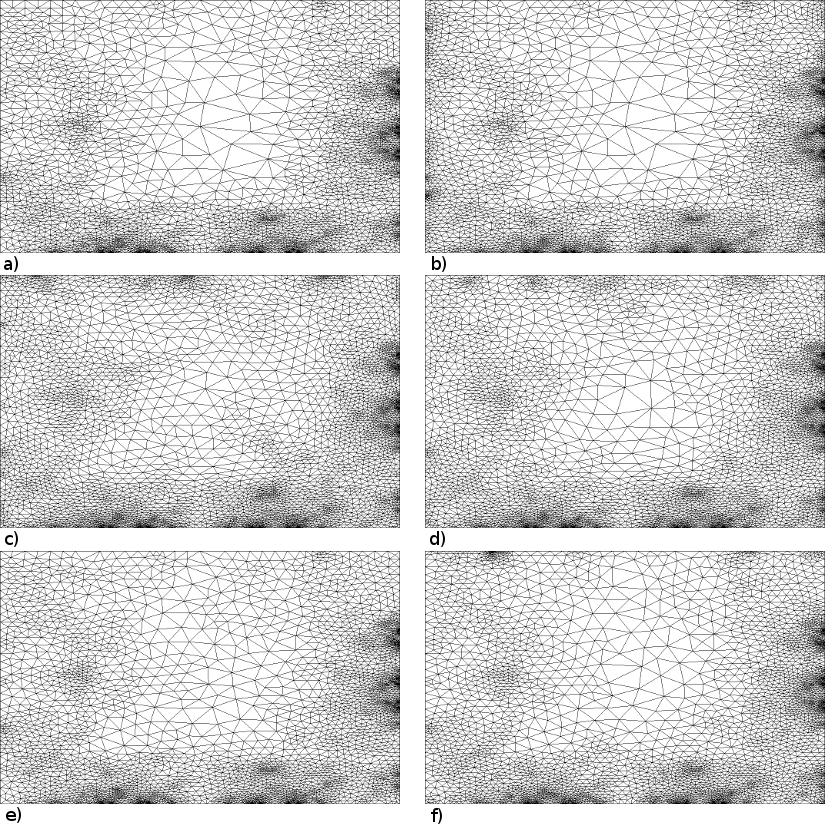
\includegraphics[width=400pt]{imagens_resultados/comparacao_movimentos.png}
  \caption{\footnotesize{Em a) malha inicial com 3.841 vértices. Em b), malha final movimentada pela função $\Lambda$; em c), pela função $\Gamma$; em d), pela função $\Xi$, em e), pela função $\Psi$ e em f), pela função $\Upsilon$.
}}
  \label{fig_comparacao_movimentos}
\end{figure}

Nas próximas subseções, apresenta-se os resultados comparativos entre as funções monitoras $\Lambda$, $\Gamma$, $\Xi$, $\Psi$ e $\Upsilon$.

\subsection{Comparativo funções monitoras}
\label{comparativo_a}

As malhas, geradas pelo algoritmo (\ref{malha_refinamento_adaptativo}), que foi configurado com número mínimo de vértices $\chi = 15.000$, $\chi = 30.000$, $\chi = 60.000$ e $\chi = 100.000$, possuem, respectivamente, um total de $15.788$, $32.515$, $67.963$ e $142.253$ vértices. Todas as malhas possuem, inicialmente, as métricas de qualidade $\rho_{max} = 1,0$ e $\upsilon_{min} = 0,6$. Na etapa temporal $t=1$, previamente ao se movimentar os vértices, o maior valor de $\gamma$, denotado $\gamma_{max}$, e o valor médio de $\gamma$, denotado $\gamma_{mean}$, das malhas geradas, encontram-se resumidos na tabela (\ref{tabela_malha_inicial}). O valor de $\gamma_{mean}$ tende a diminuir ao avançar a etapa temporal. A cada iteração do laço enquanto, linhas \ref{laco_enquanto_inicio} a \ref{laco_enquanto_fim}, do algoritmo (\ref{malha_refinamento_adaptativo}) aumenta-se o valor de $\gamma_{mean}$, inserindo-se novos vértices nas regiões de maior variação. Realizar o movimento dos vértices em direção à região de maior variação também aumenta o valor de $\gamma_{mean}$.

\begin{table}[!ht]
\begin{center}
 %aqui centralizamos a tabela
\begin{tabular}{|l|l|l|l|l|} %-----dividir em sete colunas
\hline
$\chi$ & 15.000 & 30.000 & 60.000 & 100.000 \\
\hline %----- linha horizontal
 $\gamma_{max}$    & 30,25185 & 30,91983 & 45,65052 &  65,18423\\
 $\gamma_{mean}$   & 3,08635 & 3,58712 & 4,08809 &  4,47127\\
\hline %----- linha horizontal
\end{tabular}%--- fechamento do ambiente tabular
\end{center}
 %fim da centralização da tabela
\caption{Valores de $\gamma_{max}$ e $\gamma_{mean}$, respectivamente, o maior valor de $\gamma$ e o valor médio de $\gamma$, na etapa temporal $t=1$.} %legenda da tabela
\label{tabela_malha_inicial}
\end{table}

\begin{sidewaystable}
% \scalefont{0.7}
\begin{center}
 %aqui centralizamos a tabela
\begin{tabular}{|c|l|r|r|r|r|r|r|r|} %-----dividir em sete colunas
\hline
& Função & $\Lambda$ & $\Gamma$ & $\Xi$ & $\Psi$ & $\Upsilon$ & S/Mov.1 & S/Mov.2 \\
\hline %----- linha horizontal
\multirow{5}{*}{\begin{sideways}$\chi = 15.000$\end{sideways} } 
& Total de vértices                                                     & 16.255 & 16.618 & 16.615 & 16.481 & 17.060 & 15.788 & 32.515 \\
& {\it Clocks} exp.	                                             	& 5,34e10 & 1,78e10 & 6,71e10 & 6,43e10 & 2,71e10 & 1,33e09 & 4,05e09 \\
& {\it Clocks} para mov.                                      		& 6,00e09 & 1,32e09 & 9,08e09 & 8,62e09 & 2,84e09 & - & - \\
& Rep. linhas \ref{laco_repita_inicio}-\ref{laco_repita_fim} 		& 163 & 24 & 344 & 267 & 49 & - & - \\
& Valor $\gamma_{max}$							& 128,89 & 26,39 & 26,26  & 26,21 & 180,42 & 26,13 & 36,13 \\
& Valor $\gamma_{mean}$							& 1,02420 & 0,99315 & 0,99602 & 0,99759 & 0,99436& 0,98318 & 1,03107 \\
\hline %----- linha horizontal
\multirow{5}{*}{\begin{sideways}$\chi = 30.000$\end{sideways} } 
& Total de vértices                                                     & 33.034 & 33.790 & 33.755 & 33.551 & 33.908 & 32.515 & 67.963 \\
& {\it Clocks} exp.	                                             	& 1,03e11 & 5,12e10 & 1,33e11 & 1,23e11 & 6,25e10 & 4,05e09 & 1,53e10 \\
& {\it Clocks} para mov.                                      		& 7,97e09 & 2,96e09 & 1,35e10 & 1,19e10 & 4,27e09 & - & - \\
& Rep. linhas \ref{laco_repita_inicio}-\ref{laco_repita_fim} 		& 105 & 26 & 291 & 183 & 37 & - & - \\
& Valor $\gamma_{max}$							& 50,36 & 51,24 & 50,21  & 49,43 & 111,51 & 36,13 & 52,37 \\
& Valor $\gamma_{mean}$							& 1,06513 & 1,05096 & 1,05477 & 1,05560 & 1,05921 & 1,03107 & 1,06202 \\
\hline %----- linha horizontal
\multirow{5}{*}{\begin{sideways}$\chi = 60.000$\end{sideways} } 
& Total de vértices                                                     & 68.840& 70.224 & 69.926 & 70.076 & 70.498 & 67.963 & 142.253 \\
& {\it Clocks} exp.	                                             	& 2,84e11 & 1,48e11 & 3,36e11 & 3,51e11 & 1,51e11 & 1,53e10  & 5,30e10 \\
& {\it Clocks} para mov.                                      		& 1,69e10 & 6,49e09 & 2,43e10 & 2,60e10 & 6,81e09 & - & - \\
& Rep. linhas \ref{laco_repita_inicio}-\ref{laco_repita_fim} 		& 109 & 27 & 180 & 215 & 31 & - & - \\
& Valor $\gamma_{max}$							& 177,60 & 49,47 & 52,24 & 52,35 & 174,41 & 52,37 & 72,37 \\
& Valor $\gamma_{mean}$							& 1,12378 & 1,09497 & 1,09474 & 1,09483 & 1,09755 &  1,06202 & 1,11495 \\
\hline %----- linha horizontal
\multirow{5}{*}{\begin{sideways}$\chi = 100.000$\end{sideways} } 
& Total de vértices                                                     & 143.107 & 145.346 & 145.130 & 145.163 & 146.585 & 142.253 & 298.574 \\
& {\it Clocks} exp.	                                             	& 6,00e11 & 3,80e11 & 6,25e11 & 6,26e11 & 4,36e11 & 5,30e10 & 2,18e11 \\
& {\it Clocks} para mov.                                      		& 2,30e10 & 9,66e09 & 2,84e10 & 2,92e10 & 1,27e10 & - & - \\
& Rep. linhas \ref{laco_repita_inicio}-\ref{laco_repita_fim} 		& 71 & 20 & 92 & 93 & 28 & - & - \\
& Valor $\gamma_{max}$							& 104,09 & 101,95 & 94,64 & 94,82 & 394,68 & 72,37 & 104,80 \\
& Valor $\gamma_{mean}$							& 1,12121 & 1,11986 & 1,11864 & 1,11845 & 1,12224 & 1,11495 & 1,13468 \\
\hline %----- linha horizontal
\end{tabular}%--- fechamento do ambiente tabular
\end{center}
 %fim da centralização da tabela
\caption{Comparativo das funções executadas com $\beta = 0,1$, utilizando malhas geradas pelo algoritmo (\ref{malha_refinamento_adaptativo}), configurado com $\chi = 15.000$, $\chi = 30.000$, $\chi = 60.000$ e $\chi = 100.000$, que possuem, inicialmente e respectivamente, um total de $15.788$, $32.515$, $67.963$ e $142.253$ vértices.} %legenda da tabela
\label{tabelaComparativo_beta_1}
\end{sidewaystable}

\begin{sidewaystable}
% \scalefont{0.7}
\begin{center}
 %aqui centralizamos a tabela
\begin{tabular}{|c|l|r|r|r|r|r|r|r|} %-----dividir em sete colunas
\hline
& Função & $\Lambda$ & $\Gamma$ & $\Xi$ & $\Psi$ & $\Upsilon$ & S/Mov.1 & S/Mov.2 \\
\hline %----- linha horizontal
\multirow{5}{*}{\begin{sideways}$\chi = 15.000$\end{sideways} } 
& Total de vértices                                                     & 16.263 & 17.077 & 16.596 & 16.589 & 16.785 & 15.788 & 32.515 \\
& {\it Clocks} exp.	                                             	& 2,82e10 & 1,55e10 & 2,73e10 & 2,63e10 & 1,61e10 & 1,33e09 & 4,05e09\\
& {\it Clocks} para mov.                                      		& 2,70e09 & 1,04e09 &3,01e09  & 2,85e09 & 1,05e09 & - & - \\
& Rep. linhas \ref{laco_repita_inicio}-\ref{laco_repita_fim} 		& 80 & 19 & 73 & 70 & 20 & - & - \\
& Valor $\gamma_{max}$							& 237,75 & 48,50 & 26.22 & 26.21 & 218,35 & 26,13 & 36,13 \\
& Valor $\gamma_{mean}$							& 1,02373 & 0,97805 & 0.99631 & 0,99664 & 1.02131 & 0,98318 & 1,03107 \\
\hline %----- linha horizontal
\multirow{5}{*}{\begin{sideways}$\chi = 30.000$\end{sideways} } 
& Total de vértices                                                     & 33.182 & 34.069 & 33.775 & 33.770 & 34.284 & 32.515 & 67.963 \\
& {\it Clocks} exp.	                                             	& 6,91e10 & 4,13e10 & 6,81e10 & 6,82e10 & 4,27e10 & 4,05e09 & 1,53e10 \\
& {\it Clocks} para mov.                                      		& 4,63e09 & 1,91e09 & 5,92e09 & 5,57e09 & 1,94e09 & - & - \\
& Rep. linhas \ref{laco_repita_inicio}-\ref{laco_repita_fim} 		& 61 & 17 & 69 & 69 & 18 & - & - \\
& Valor $\gamma_{max}$							& 99,92 & 53,50 & 50,17 & 50,18 & 105,29 & 36,13 & 52,37 \\
& Valor $\gamma_{mean}$							& 1,07718 & 1,04963 & 1,05470 & 1,05460 & 1,06094 & 1,03107 & 1,06202 \\
\hline %----- linha horizontal
\multirow{5}{*}{\begin{sideways}$\chi = 60.000$\end{sideways} } 
& Total de vértices                                                     & 68.789 & 70.889 & 70.003 & 69.997 & 71.222 & 67.963 & 142.253 \\
& {\it Clocks} exp.	                                             	& 1,76e11 & 1,23e11 & 1,67e11 & 1,66e11 & 1,30e11 & 1,53e10 &  5,30e10 \\
& {\it Clocks} para mov.                                  		& 8,39e09 & 3,79e09 & 8,46e09 & 8,41e09 & 4,69e09 & - & - \\
& Rep. linhas \ref{laco_repita_inicio}-\ref{laco_repita_fim} 		& 64 & 16 & 45 & 45 & 20 & - & - \\
& Valor $\gamma_{max}$							& 221,19 & 151,52 & 52,25 & 52.26 & 221,87 & 52,37 & 72,37 \\
& Valor $\gamma_{mean}$							& 1,10905 & 1,09070 & 1.09452 & 1.09468 & 1,09799 & 1,06202 & 1,11495 \\
\hline %----- linha horizontal
\multirow{5}{*}{\begin{sideways}$\chi = 100.000$\end{sideways} } 
& Total de vértices                                                     & 143.319 & 145.768 & 145.355 & 145.352 & 147.731 & 142.253 & 298.574 \\
& {\it Clocks} exp.	                                             	& 3,95e11 & 3,08e11 & 3,72e11 & 3,73e11 & 3,59e11 & 5,30e10 & 2,18e11 \\
& {\it Clocks} para mov.                                      		& 1,22e10 & 5,33e09 & 1,17e10 & 1,12e10 & 8,99e09 & - & - \\
& Rep. linhas \ref{laco_repita_inicio}-\ref{laco_repita_fim} 		& 45 & 11 & 25 & 25 & 19 & - & - \\
& Valor $\gamma_{max}$							& 108,01 & 102,34 & 95,79 & 95,81 & 135,68 & 72,37 & 104,80 \\
& Valor $\gamma_{mean}$							& 1,12327 & 1,12005 & 1,11871 & 1,11870 & 1,12471 & 1,11495 & 1,13468 \\
\hline %----- linha horizontal
\end{tabular}%--- fechamento do ambiente tabular
\end{center}
 %fim da centralização da tabela
\caption{Comparativo das funções executadas com $\beta = 0,2$, utilizando malhas geradas pelo algoritmo (\ref{malha_refinamento_adaptativo}), configurado com $\chi = 15.000$, $\chi = 30.000$, $\chi = 60.000$ e $\chi = 100.000$. que possuem, inicialmente e respectivamente, um total de $15.788$, $32.515$, $67.963$ e $142.253$ vértices.} %legenda da tabela
\label{tabelaComparativo_beta_2}
\end{sidewaystable}


\begin{sidewaystable}
% \scalefont{0.7}
\begin{center}
 %aqui centralizamos a tabela
\begin{tabular}{|c|l|r|r|r|r|r|r|r|} %-----dividir em sete colunas
\hline
& Função & $\Lambda$ & $\Gamma$ & $\Xi$ & $\Psi$ & $\Upsilon$ & S/Mov.1 & S/Mov.2 \\
\hline %----- linha horizontal
\multirow{5}{*}{\begin{sideways}$\chi = 15.000$\end{sideways} } 
& Total de vértices                                                     & 16.252 & 16.928 & 16.911 & 16.889 & 17.362 & 15.788 & 32.515 \\
& {\it Clocks} exp.	                                             	& 1,93e10 & 1,18e10 & 2,07e10 & 2,08e10 & 1,49e10 & 1,33e09 & 4,05e09\\
& {\it Clocks} para mov.                                      		& 1,47e09 & 5,72e08 & 2,04e09 &  2,08e09& 9,19e08 & - & - \\
& Rep. linhas \ref{laco_repita_inicio}-\ref{laco_repita_fim} 		& 35 & 10 & 50 & 50 & 18 & - & - \\
& Valor $\gamma_{max}$							& 50,62 & 25,05 & 26,34 & 26,35 & 226,14 & 26,13 & 36,13 \\
& Valor $\gamma_{mean}$							& 1,03007 & 0,98279 & 0,98485 & 0,98614 & 1,00625 & 0,98318 & 1,03107 \\
\hline %----- linha horizontal
\multirow{5}{*}{\begin{sideways}$\chi = 30.000$\end{sideways} } 
& Total de vértices                                                     & 33.094 & 34.521 & 34.005 & 34.007 & 34.605 & 32.515 & 67.963 \\
& {\it Clocks} exp.	                                             	& 5,04e10 & 3,82e10 & 5,16e10 & 5,19e10 & 3,99e10 & 4,05e09 & 1,53e10 \\
& {\it Clocks} para mov.                                      		& 2,82e09 & 1,56e09 & 3,75e09 & 3,70e09 & 1,82e09 & - & - \\
& Rep. linhas \ref{laco_repita_inicio}-\ref{laco_repita_fim} 		& 31 & 13 & 40 & 40 & 15 & - & - \\
& Valor $\gamma_{max}$							& 103,83 & 53,56 & 50,58 & 50,59 & 184,96 & 36,13 & 52,37 \\
& Valor $\gamma_{mean}$							& 1,06771 & 1,04496 & 1,05362 & 1,05377 & 1,05276 & 1,03107 & 1,06202 \\
\hline %----- linha horizontal
\multirow{5}{*}{\begin{sideways}$\chi = 60.000$\end{sideways} } 
& Total de vértices                                                     & 68.904 & 71.040 & 70.587 & 70.588 & 71.576 & 67.963 & 142.253 \\
& {\it Clocks} exp.	                                             	& 1,48e11 & 1,07e11 & 1,35e11 & 1,35e11 & 1,11e11 & 1,53e10 &  5,30e10 \\
& {\it Clocks} para mov.                                  		& 6,26e09 & 2,92e09 & 6,29e09 & 5,95e09 & 3,28e09 & - & - \\
& Rep. linhas \ref{laco_repita_inicio}-\ref{laco_repita_fim} 		& 49 & 12 & 32 & 32 & 14 & - & - \\
& Valor $\gamma_{max}$							& 207,01 & 75,58 & 52,55 & 52,56 & 221,22 & 52,37 & 72,37 \\
& Valor $\gamma_{mean}$							& 1,11019 & 1,09184 & 1,09593 & 1,09592 & 1,09860 & 1,06202 & 1,11495 \\
\hline %----- linha horizontal
\multirow{5}{*}{\begin{sideways}$\chi = 100.000$\end{sideways} } 
& Total de vértices                                                     & 143.316 & 147.723 & 146.457 & 146.452 & 147.899 & 142.253 & 298.574 \\
& {\it Clocks} exp.	                                             	& 3,65e11 & 3,40e11 & 3,52e11 & 3,51e11 & 3,33e11 & 5,30e10 & 2,18e11 \\
& {\it Clocks} para mov.                                      		& 8,88e09 & 6,97e09 & 8,82e09 & 9,52e09 & 5,74e09 & - & - \\
& Rep. linhas \ref{laco_repita_inicio}-\ref{laco_repita_fim} 		& 30 & 13 & 19 & 19 & 12 & - & - \\
& Valor $\gamma_{max}$							& 107,99 & 90,95 & 98,87 & 98,88 & 224,65 & 72,37 & 104,80 \\
& Valor $\gamma_{mean}$							& 1,12210 & 1,11902 & 1,11867 & 1,11870 & 1,12318 & 1,11495 & 1,13468 \\
\hline %----- linha horizontal
\end{tabular}%--- fechamento do ambiente tabular
\end{center}
 %fim da centralização da tabela
\caption{Comparativo das funções executadas com $\beta = 0,3$, utilizando malhas geradas pelo algoritmo (\ref{malha_refinamento_adaptativo}), configurado com $\chi = 15.000$, $\chi = 30.000$, $\chi = 60.000$ e $\chi = 100.000$. que possuem, inicialmente e respectivamente, um total de $15.788$, $32.515$, $67.963$ e $142.253$ vértices.} %legenda da tabela
\label{tabelaComparativo_beta_3}
\end{sidewaystable}

\begin{sidewaystable}
% \scalefont{0.7}
\begin{center}
 %aqui centralizamos a tabela
\begin{tabular}{|c|l|r|r|r|r|r|r|r|} %-----dividir em sete colunas
\hline
& Função & $\Lambda$ & $\Gamma$ & $\Xi$ & $\Psi$ & $\Upsilon$ & S/Mov.1 & S/Mov.2 \\
\hline %----- linha horizontal
\multirow{5}{*}{\begin{sideways}$\chi = 15.000$\end{sideways} } 
& Total de vértices                                                     & 16.701 & 17.579 & 16.837 & 16.821 & 17.355 & 15.788 & 32.515 \\
& {\it Clocks} exp.	                                             	& 1,62e10 & 1,27e10 & 1,55e10 & 1,56e10 & 1,32e10 & 1,33e09 & 4,05e09\\
& {\it Clocks} para mov.                                      		& 1,14e09 & 6,37e08 & 1,22e09 & 1,28e09 & 7,26e08 & - & - \\
& Rep. linhas \ref{laco_repita_inicio}-\ref{laco_repita_fim} 		& 30 & 11 & 26 & 25 & 13 & - & - \\
& Valor $\gamma_{max}$							& 388,50 & 58,95 & 26,29 & 26,28 & 211,07 & 26,13 & 36,13 \\
& Valor $\gamma_{mean}$							& 1,14899 & 0,96986 & 0,99102 & 0,99077 & 1,01422 & 0,98318 & 1,03107 \\
\hline %----- linha horizontal
\multirow{5}{*}{\begin{sideways}$\chi = 30.000$\end{sideways} } 
& Total de vértices                                                     & 33.315 & 34.980 &  34.391 & 34.381 & 34.746 & 32.515 & 67.963 \\
& {\it Clocks} exp.	                                             	& 4,27e10 & 3,54e10 & 4,47e10 & 4,50e10 & 3,69e10 & 4,05e09 & 1,53e10 \\
& {\it Clocks} para mov.                                      		& 1,88e09 & 1,13e09 & 2,67e09 & 2,51e09 & 1,29e09 & - & - \\
& Rep. linhas \ref{laco_repita_inicio}-\ref{laco_repita_fim} 		& 21 & 10 & 29 & 29 & 11 & - & - \\
& Valor $\gamma_{max}$							& 224,84 & 65,94 & 50,86 &  50,85 & 215,36 & 36,13 & 52,37 \\
& Valor $\gamma_{mean}$							& 1,11159 & 1,04457 & 1,04929 & 1,04969 & 1,05862 & 1,03107 & 1,06202 \\
\hline %----- linha horizontal
\multirow{5}{*}{\begin{sideways}$\chi = 60.000$\end{sideways} } 
& Total de vértices                                                     & 68.846 & 71.937 & 71.170 & 71.125 & 72.224 & 67.963 & 142.253 \\
& {\it Clocks} exp.	                                             	& 1,22e11 & 1,06e11 & 1,18e11 & 1,17e11 & 1,07e11 & 1,53e10 &  5,30e10 \\
& {\it Clocks} para mov.                                      		& 4,39e09 & 2,50e09 & 4,39e09 & 4,41e09 & 2,63e09 & - & - \\
& Rep. linhas \ref{laco_repita_inicio}-\ref{laco_repita_fim} 		& 24 & 11 & 21 & 20 & 11 & - & - \\
& Valor $\gamma_{max}$							& 227,53 & 106,15 & 52,68 & 52,64 & 365,12 & 52,37 & 72,37 \\
& Valor $\gamma_{mean}$							& 1,10886 & 1,09097 & 1,09448 & 1,09445 & 1,10247 & 1,06202 & 1,11495 \\
\hline %----- linha horizontal
\multirow{5}{*}{\begin{sideways}$\chi = 100.000$\end{sideways} } 
& Total de vértices                                                     & 143.306 & 149.079 & 147.478 & 147.508 & 148.898 & 142.253 & 298.574 \\
& {\it Clocks} exp.	                                             	& 3,48e11 & 3,33e11 & 3,42e11 & 3,41e11 & 3,20e11 & 5,30e10 & 2,18e11 \\
& {\it Clocks} para mov.                                      		& 7,48e09 & 5,87e09 & 7,93e09 & 8,20e09 & 5,07e09 & - & - \\
& Rep. linhas \ref{laco_repita_inicio}-\ref{laco_repita_fim} 		& 19 & 12 & 16 & 16 & 10 & - & - \\
& Valor $\gamma_{max}$							& 298,82 & 387,05 & 100,34 & 100,35 & 212,82 & 72,37 & 104,80 \\
& Valor $\gamma_{mean}$							& 1,12429 & 1,12151 & 1,11912 & 1,11908 & 1,12472 & 1,11495 & 1,13468 \\
\hline %----- linha horizontal
\end{tabular}%--- fechamento do ambiente tabular
\end{center}
 %fim da centralização da tabela
\caption{Comparativo das funções executadas com $\beta = 0,4$, utilizando malhas geradas pelo algoritmo (\ref{malha_refinamento_adaptativo}), configurado com $\chi = 15.000$, $\chi = 30.000$, $\chi = 60.000$ e $\chi = 100.000$. que possuem, inicialmente e respectivamente, um total de $15.788$, $32.515$, $67.963$ e $142.253$ vértices.} %legenda da tabela
\label{tabelaComparativo_beta_4}
\end{sidewaystable}

\begin{sidewaystable}
% \scalefont{0.7}
\begin{center}
 %aqui centralizamos a tabela
\begin{tabular}{|c|l|r|r|r|r|r|r|r|} %-----dividir em sete colunas
\hline
& Função & $\Lambda$ & $\Gamma$ & $\Xi$ & $\Psi$ & $\Upsilon$ & S/Mov.1 & S/Mov.2 \\
\hline %----- linha horizontal
\multirow{5}{*}{\begin{sideways}$\chi = 15.000$\end{sideways} } 
& Total de vértices                                                     & 16.917 & 18.196 & 17.172 & 17.281 & 17.933 & 15.788 & 32.515 \\
& {\it Clocks} exp.	                                             	& 1,50e10 & 1,29e10 & 1,44e10 & 1,46e10 & 1,30e10 & 1,33e09 & 4,05e09 \\
& {\it Clocks} para mov.                                      		& 4,24e08 & 5,98e08 & 9,41e08 & 9,67e08 & 6,16e08 & - & - \\
& Rep. linhas \ref{laco_repita_inicio}-\ref{laco_repita_fim} 		& 10 & 10 & 19 & 20 & 11 & - & - \\
& Valor $\gamma_{max}$							& 67,98 & 50,23 & 26,38 & 26,40 & 447,48 & 26,13 & 36,13 \\
& Valor $\gamma_{mean}$							& 1,04517 & 0,95807 & 0,98742 & 0,98068 & 1,04418 & 0,98318 & 1,03107 \\
\hline %----- linha horizontal
\multirow{5}{*}{\begin{sideways}$\chi = 30.000$\end{sideways} } 
& Total de vértices                                                     & 33.852 & 35.659 & 34.639 & 34.640 & 35.215 & 32.515 & 67.963 \\
& {\it Clocks} exp.	                                             	& 4,17e10 & 3,78e10 & 4,16e10 & 4,13e10 & 3,59e10 & 4,05e09 & 1,53e10 \\
& {\it Clocks} para mov.                                      		& 1,60e09 & 1,23e09 & 2,20e09 & 2,04e09 & 1,09e09 & - & - \\
& Rep. linhas \ref{laco_repita_inicio}-\ref{laco_repita_fim} 		& 16 & 11 & 20 & 20 & 10 & - & - \\
& Valor $\gamma_{max}$							& 219,21 & 48,97 & 51,01 & 51,02 & 374,23 & 36,13 & 52,37 \\
& Valor $\gamma_{mean}$							& 1,09169 & 1,03820 & 1,05415 & 1,05422 & 1,05477 & 1,03107 & 1,06202 \\
\hline %----- linha horizontal
\multirow{5}{*}{\begin{sideways}$\chi = 60.000$\end{sideways} } 
& Total de vértices                                                     & 69.059 & 72.892 & 71.639 & 71.622 & 74.041 & 67.963 & 142.253 \\
& {\it Clocks} exp.	                                             	& 1,18e11 & 1,06e11 & 1,10e11 & 1,10e11 & 1,11e11 & 1,53e10  & 5,30e10 \\
& {\it Clocks} para mov.                                      		& 4,07e09 & 2,38e09 & 3,32e09 & 3,34e09 & 3,01e09 & - & - \\
& Rep. linhas \ref{laco_repita_inicio}-\ref{laco_repita_fim} 		& 25 & 10 & 14 & 14 & 12 & - & - \\
& Valor $\gamma_{max}$							& 417,86 & 104,08 & 67,41 & 67.42 & 758,03 & 52,37 & 72,37 \\
& Valor $\gamma_{mean}$							& 1,12834 & 1,08956 & 1,09577 & 1,09572 & 1,11319 &  1,06202 & 1,11495 \\
\hline %----- linha horizontal
\multirow{5}{*}{\begin{sideways}$\chi = 100.000$\end{sideways} } 
& Total de vértices                                                     & 143.497 & 150.672 & 148.841 & 148.791 & 151.400 & 142.253 & 298.574 \\
& {\it Clocks} exp.	                                             	& 3,36e11 & 3,25e11 & 3,28e11 & 3,29e11 & 3,30e11 & 5,30e10 & 2,18e11 \\
& {\it Clocks} para mov.                                      		& 6,49e09 & 5,05e09 & 6,02e09 & 6,00e09 & 5,51e09 & - & - \\
& Rep. linhas \ref{laco_repita_inicio}-\ref{laco_repita_fim} 		& 17 & 10 & 12 & 12 & 10 & - & - \\
& Valor $\gamma_{max}$							& 202,91 & 99,86 & 100,82 & 100,83 & 723,86 & 72,37 & 104,80 \\
& Valor $\gamma_{mean}$							& 1,12883 & 1,11895 & 1,11961 & 1,11971 & 1,13135 & 1,11495 & 1,13468 \\
\hline %----- linha horizontal
\end{tabular}%--- fechamento do ambiente tabular
\end{center}
 %fim da centralização da tabela
\caption{Comparativo das funções executadas com $\beta = 0,5$, utilizando malhas geradas pelo algoritmo (\ref{malha_refinamento_adaptativo}), configurado com $\chi = 15.000$, $\chi = 30.000$, $\chi = 60.000$ e $\chi = 100.000$, que possuem, inicialmente e respectivamente, um total de $15.788$, $32.515$, $67.963$ e $142.253$ vértices.} %legenda da tabela
\label{tabelaComparativo_beta_5}
\end{sidewaystable}


\begin{sidewaystable}
% \scalefont{0.7}
\begin{center}
 %aqui centralizamos a tabela
\begin{tabular}{|c|l|r|r|r|r|r|r|r|} %-----dividir em sete colunas
\hline
& Função & $\Lambda$ & $\Gamma$ & $\Xi$ & $\Psi$ & $\Upsilon$ & S/Mov.1 & S/Mov.2 \\
\hline %----- linha horizontal
\multirow{5}{*}{\begin{sideways}$\chi = 15.000$\end{sideways} } 
& Total de vértices                                                     & - & 19.997 & 18.528 & 18.517 & 18.614 & 15.788 & 32.515 \\
& {\it Clocks} exp.	                                             	& - & 1,40e10 & 1,37e10 & 1,36e10 & 1,35e10 & 1,33e09 & 4,05e09 \\
& {\it Clocks} para mov.                                      		& - & 6,32e08 & 6,49e08 & 6,51e08 & 5,93e08 & - & - \\
& Rep. linhas \ref{laco_repita_inicio}-\ref{laco_repita_fim} 		& - & 10 & 11 & 11 & 10 & - & - \\
& Valor $\gamma_{max}$							& - & 97,91 & 26,25 & 26.26 & 399,67 & 26,13 & 36,13 \\
& Valor $\gamma_{mean}$							& - & 0,91555 & 0,99277 & 0,99308 & 1,03788 & 0,98318 & 1,03107 \\
\hline %----- linha horizontal
\multirow{5}{*}{\begin{sideways}$\chi = 30.000$\end{sideways} } 
& Total de vértices                                                     & - & 38.077 & 37.604 & 37.690 & 37.550 & 32.515 & 67.963 \\
& {\it Clocks} exp.	                                             	& - & 3,23e10 & 2,42e10 & 3,21e10 & 2,44e10 & 4,05e09 & 1,53e10 \\
& {\it Clocks} para mov.                                      		& - & 1,00e09 & 7,06e08 & 9,50e08 & 7,39e08 & - & - \\
& Rep. linhas \ref{laco_repita_inicio}-\ref{laco_repita_fim} 		& - & 10 & 10 & 10 & 10 & - & - \\
& Valor $\gamma_{max}$							& - & 215,22 & 50,59 & 50,60 & 717,38 & 36,13 & 52,37 \\
& Valor $\gamma_{mean}$							& - & 1,01722 & 1,04631 & 1,04435 & 1,07486 & 1,03107 & 1,06202 \\
\hline %----- linha horizontal
\multirow{5}{*}{\begin{sideways}$\chi = 60.000$\end{sideways} } 
& Total de vértices                                                     & - & 77.253 & 77.471 & 77.536 & 77.250 & 67.963 & 142.253 \\
& {\it Clocks} exp.	                                             	& - & 1,15e11 & 1,14e11 & 1,16e11 & 1,17e11 & 1,53e10  & 5,30e10 \\
& {\it Clocks} para mov.                                      		& - & 2,64e09 & 2,67e09 & 2,44e09 & 2,51e09 & - & - \\
& Rep. linhas \ref{laco_repita_inicio}-\ref{laco_repita_fim} 		& - & 10 & 10 & 10 & 10 & - & - \\
& Valor $\gamma_{max}$							& - & 371,55 & 52,58 & 52,59 & 1.427,98 & 52,37 & 72,37 \\
& Valor $\gamma_{mean}$							& - & 1,07850 & 1,09331 & 1.09449 & 1,11611 &  1,06202 & 1,11495 \\
\hline %----- linha horizontal
\multirow{5}{*}{\begin{sideways}$\chi = 100.000$\end{sideways} } 
& Total de vértices                                                     & - & 157.280 & 162.631 & 162.660 & 157.798 & 142.253 & 298.574 \\
& {\it Clocks} exp.	                                             	& - & 3,54e11 & 3,61e11 & 3,62e11 & 3,59e11 & 5,30e10 & 2,18e11 \\
& {\it Clocks} para mov.                                      		& - & 5,46e09 & 5,36e09 & 5,18e09 & 5,04e09 & - & - \\
& Rep. linhas \ref{laco_repita_inicio}-\ref{laco_repita_fim} 		& - & 10 & 10 & 10 & 10 & - & - \\
& Valor $\gamma_{max}$							& - & 353,98 & 105,56 & 105.57 & 2.236,51 & 72,37 & 104,80 \\
& Valor $\gamma_{mean}$							& - & 1,11889 & 1,11625 & 1,11611 & 1,14206 & 1,11495 & 1,13468 \\
\hline %----- linha horizontal
\end{tabular}%--- fechamento do ambiente tabular
\end{center}
 %fim da centralização da tabela
\caption{Comparativo das funções executadas com $\beta = 0,6$, utilizando malhas geradas pelo algoritmo (\ref{malha_refinamento_adaptativo}), configurado com $\chi = 15.000$, $\chi = 30.000$, $\chi = 60.000$ e $\chi = 100.000$, que possuem, inicialmente e respectivamente, um total de $15.788$, $32.515$, $67.963$ e $142.253$ vértices. A função $\Lambda$ apresentou emaranhamentos em todos os experimentos e, para malha inicial com $32.515$ vértices, todas as funções monitoras apresentaram emaranhamentos.} %legenda da tabela
\label{tabelaComparativo_beta_6}
\end{sidewaystable}

Pode-se verificar nas tabelas (\ref{tabelaComparativo_beta_1}) a (\ref{tabelaComparativo_beta_6}) os valores gerais comparativos executando-se o algoritmo (\ref{malha_movel}) para cada função monitora. Utilizaram-se malhas geradas pelo algoritmo (\ref{malha_refinamento_adaptativo}), com $15.788$, $32.515$, $67.963$ e $142.253$ vértices, que são movimentadas  pelo algoritmo (\ref{malha_movel}), utilizando-se $\beta = 0,1$, $\beta = 0,2$, $\beta = 0,3$, $\beta = 0,4$, $\beta = 0,5$ e $\beta = 0,6$. Nessas tabelas, nas linhas rotuladas ``Total de vértices'', tem-se o total de vértices no fim da execução do algoritmo (\ref{malha_movel}), que realiza o movimento dos vértices e a melhoria da qualidade da malha. Nas linhas rotuladas ``{\it Clocks} exp.'' tem-se o total de {\it clocks} para execução total do experimento. Nas linhas rotuladas ``{\it Clocks} para mov.'', tem-se o total de {\it clocks} para movimentar os vértices, linha \ref{movimenta_malha} do algoritmo (\ref{malha_movel}). Nas linhas rotuladas ``Rep. linhas \ref{laco_repita_inicio}-\ref{laco_repita_fim}'', apresenta-se o total de repetições das linhas \ref{laco_repita_inicio} a \ref{laco_repita_fim} do algoritmo (\ref{malha_movel}). Nas linhas rotuladas ``Valor $\gamma_{max}$'', tem-se o valor de $\gamma_{max}$ no fim do experimento. E, nas linhas rotuladas ``Valor $\gamma_{mean}$'', expõe-se o valor de $\gamma_{mean}$ da malha.

Na penúltima coluna das tabelas (\ref{tabelaComparativo_beta_1}) a (\ref{tabelaComparativo_beta_6}), rotulada ``S/Mov.1'', apresentam-se os resultados obtidos avançando as dez etapas temporais para cada uma das malhas iniciais, geradas pelo algoritmo (\ref{malha_refinamento_adaptativo}), sem movimentar os vértices, configuradas com os valores de entrada conforme a tabela (\ref{tabelaValorParametros}). Na última coluna dessas tabelas, rotulada ``S/Mov.2'', apresentam-se os resultados obtidos avançando as dez etapas temporais, sem movimentar os vértices, utilizando uma malha com uma maior quantidade de vértices. 

Com os dados da penúltima coluna, das tabelas (\ref{tabelaComparativo_beta_1}) a (\ref{tabelaComparativo_beta_6}), confirma-se que movimentar os vértices aumenta o valor do gradiente, conforme pode-se verificar os valores de $\gamma_{max}$ e $\gamma_{mean}$. No entanto, em alguns resultados os valores de $\gamma_{max}$ foram menores que o experimento ``S/Mov.1'', como por exemplo nas funções $\Xi$ e $\Psi$ com $\chi = 60.000$, $\beta = 0,1$ e $\beta = 0,2$. Acredita-se que a etapa de movimento negativo dessas funções, controlado por $\mu$,  afetou os triângulos com maiores valores de $\gamma$ da malha. Nota-se também que, no caso da função $\Gamma$, no experimento $\chi = 60.000$ e $\beta = 0,1$, também obteve-se valor de $\gamma_{max}$ menor que no experimento ``S/Mov.1''.

Apresentam-se os experimentos na última coluna, das tabelas (\ref{tabelaComparativo_beta_1}) a (\ref{tabelaComparativo_beta_6}), a fim de comparar o custo do refinamento adaptativo com o custo ao se movimentar os vértices.  Em todos os experimentos, movimentar os vértices acarretou um custo computacional maior que o experimento ``S/Mov.2''. Na tabela (\ref{tabela_analise_clock}), dividiu-se o tempo de execução do experimento ``S/Mov.2'' pelo tempo de execução da função com menor custo computacional. A partir dessa tabela, verifica-se a média dessa porcentagem para cada valor de $\beta$, com arredondamento para cima. Os melhores valores foram obtidos utilizando-se $\beta = 0,6$. 

\begin{table}[!ht]
\scalefont{0.6}
\begin{center}
\begin{tabular}{ccc}
\hline
$\beta$ & $\chi$ & Percentual \\
\hline
\multirow{5}{*}{$0,1$}  
& 15.000  & 23 \% \\
& 30.000  & 30 \% \\
& 60.000  & 36 \% \\
& 100.000 & 57 \% \\
\hline              
& Média & 37 \% \\
& & \\          
\multirow{5}{*}{$0,2$}  
& 15.000  & 26  \% \\
& 30.000  & 37  \% \\
& 60.000  & 43  \% \\
& 100.000 & 71  \% \\
\hline              
& Média & 44 \% \\
& & \\        
\multirow{5}{*}{$0,3$} 
& 15.000  & 34  \% \\
& 30.000  & 40  \% \\
& 60.000  & 50  \% \\
& 100.000 & 65  \% \\
\hline              
& Média & 47 \% \\
& & \\   
\multirow{5}{*}{$0,4$} 
& 15.000  & 32 \% \\
& 30.000  & 43 \% \\
& 60.000  & 50 \% \\
& 100.000 & 68 \% \\
\hline              
& Média & 48 \% \\
& & \\   
\multirow{5}{*}{$0,5$} 
& 15.000  &  31 \% \\
& 30.000  &  42 \% \\
& 60.000  &  50 \% \\
& 100.000 &  67 \% \\
\hline              
& Média & 48 \% \\
& & \\   
\multirow{5}{*}{$0,6$} 
& 15.000  &  30 \% \\
& 30.000  &  63 \% \\
& 60.000  &  46 \% \\
& 100.000 &  61 \% \\
\hline              
& Média & 50 \% \\
\end{tabular}%--- fechamento do ambiente tabular
\end{center}
\caption{Percentagem do tempo de execução do experimento ``S/Mov.2'' em relação ao experimento com menor custo computacional ao se movimentar os vértices. Apresenta-se a média dessa percentagem para cada valor de $\beta$.}
\label{tabela_analise_clock}
\end{table}

Ainda em relação ao experimento ``S/Mov.2'', a maioria dos experimentos, em que movimentou-se os vértices, apresentou valores de $\gamma_{mean}$ relativamente próximos aos valores do experimento ``S/Mov.2'' e valores de $\gamma_{max}$ superiores, com um custo computacional também superior ao custo do experimento ``S/Mov.2''. Um motivo do valor de $\gamma_{mean}$ não ser muito superior se deve ao parâmetro $\beta$, que é definido globalmente, podendo ocorrer degeneração de triângulos localizados em regiões de baixa variação. Logo, esses triângulos necessitariam ser refinados, gerando dois novos triângulos nas regiões de baixa variação, diminuindo o valor de $\gamma_{mean}$. Provavelmente, definir um $\beta$ local apresentaria melhores resultados.

Em alguns casos, ocorreu redução dos valores de $\gamma_{max}$ e $\gamma_{mean}$ ao se utilizar malhas com mais vértices. Como por exemplo, a função $\Gamma$, no experimento $\beta = 0,2$ e $\chi = 60.000$, possuía $\gamma_{max} = 151,52$, e no experimento com $\beta = 0,2$ e $\chi = 100.000$ esse valor diminuiu para $\gamma_{max} = 102,34$. Algumas análises mostraram que, ao se movimentar os vértices, tornando-os muito próximos, os valores da EDP desses vértices serão praticamente iguais, devido à precisão definida por $\epsilon$. Com isso, triângulos que contenham esses vértices terão o valor de $\gamma$ diminuído, afetando os valores de $\gamma_{max}$ e $\gamma_{mean}$. 

Analisando-se a velocidade de execução do experimento e a quantidade de vértices nas tabelas (\ref{tabelaComparativo_beta_1}) a (\ref{tabelaComparativo_beta_5}), percebe-se que, mesmo a função $\Lambda$ obtendo a menor quantidade final de vértices em todos os experimentos,  demandou mais recursos computacionais que a função $\Gamma$ e $\Upsilon$ pois, necessitou de um número maior de iterações do laço que movimenta os vértices. Ainda, na função $\Lambda$ é necessário encontrar o maior valor de $\Delta \phi_{max}$. Entretanto, o tempo de execução é afetado principalmente pelo método dos gradientes conjugados, procedimento que mais demanda recursos, e é executado dentro do laço que movimenta os vértices. As funções $\Xi$ e $\Psi$ necessitaram de um número maior de {\it clocks} devido à combinação das duas suavizações, que torna o movimento vagaroso em relação às demais funções.

Pelos resultados das tabelas (\ref{tabelaComparativo_beta_1}) a (\ref{tabelaComparativo_beta_5}), verifica-se que a função monitora proposta, $\Lambda$, apresentou bons resultados ao se analisar a quantidade final de vértices e os valores de $\gamma_{max}$ e $\gamma_{mean}$. A função $\Gamma$ foi a que necessitou da menor quantidade de {\it clocks} de execução em quase todos os experimentos, consequência do menor número de iterações da linhas \ref{laco_repita_inicio} a \ref{laco_repita_fim} do algoritmo (\ref{malha_movel}) e, ainda, resultou em $\gamma_{max}$ e $\gamma_{mean}$ finais razoáveis. As funções $\Xi$ e $\Psi$ em todos os experimentos sempre estiveram entre os três piores resultados em relação ao número de {\it clocks} para movimentar os vértices. A função $\Upsilon$ apresentou, em dois experimentos, o melhor custo computacional, e nos demais, o segundo melhor custo computacional e, ainda, apresentou bons resultados em relação aos valores de $\gamma_{max}$ e $\gamma_{mean}$, sempre estando entre os dois melhores resultados no entanto, quanto à quantidade de vértices, obteve o pior desempenho em quase todos os experimentos. 

Na tabela (\ref{tabela_rho}), apresenta-se a média das dez iterações temporais da métrica {\it Circunradius-to-shortest Edge Radio} (CER), denotada $\rho_{max}$, após movimentar os vértices, para cada experimento realizado. Quanto maior o valor da métrica CER, pior é o resultado, pois menor é o ângulo mínimo. Os valores são agrupados para cada experimento. Nessa tabela, pode-se observar que as funções $\Psi$ e $\Xi$ apresentaram os melhores resultados e $\Gamma$ os piores, na maioria dos casos.

\begin{table}[!ht]
\begin{center}
 %aqui centralizamos a tabela
\begin{tabular}{|l|l|l|l|l|l|l|} %-----dividir em sete colunas
\hline
$\beta$ & $\chi$ & $\Lambda$ & $\Gamma$ & $\Xi$ & $\Psi$ & $\Upsilon$ \\
\hline %----- linha horizontal
\multirow{4}{*}{$0,1$}
& 15.000 & 1,15824 & 1,13563 & 1,11155 & 1,08556 & 1,14298 \\
& 30.000 & 1,08060 & 1,19005 & 1,09516 & 1,08460 & 1,12088 \\
& 60.000 & 1,12058 & 1,15848 & 1,07265 & 1,08692 & 1,12528 \\
& 100.000 & 1,07919 & 1,10902 & 1,04850 & 1,04756 & 1,10878 \\
\hline %----- linha horizontal
\multirow{4}{*}{$0,2$}
& 15.000 & 1,17876 & 1,23320 & 1,13482 & 1,13301 & 1,16649 \\
& 30.000 & 1,12482 & 1,26227 & 1,09764 & 1,10480 & 1,20191 \\
& 60.000 & 1,10528 & 1,22472 & 1,08806 & 1,09810 & 1,16519\\
& 100.000 & 1,12786 & 1,13104 & 1,06125 & 1,06139 & 1,16649 \\
\hline %----- linha horizontal
\multirow{4}{*}{$0,3$}
& 15.000 & 1,20717 & 1,24393 & 1,19507 & 1,20842 & 1,22321 \\
& 30.000 & 1,16724 & 1,31336 & 1,12671 & 1,11300 & 1,19550 \\
& 60.000 & 1,14563 & 1,32805 & 1,11670 & 1,11709 & 1,24962 \\
& 100.000 & 1,15702 & 1,26131 & 1,08974 & 1,08982 & 1,19858 \\
\hline %----- linha horizontal
\multirow{4}{*}{$0,4$}
& 15.000 & 1,44468 & 1,33633 & 1,19630 & 1,19693 & 1,21874 \\
& 30.000 & 1,39521 & 1,31444 & 1,25018 & 1,25135 & 1,22399 \\
& 60.000 & 1,26923 & 1,37858 & 1,16041 & 1,15642 & 1,24856 \\
& 100.000 & 1,14348 & 1,34365 & 1,14234 & 1,14245 & 1,26469 \\
\hline %----- linha horizontal
\multirow{4}{*}{$0,5$}
& 15.000 & 6,17023 & 1,49158 & 1,28772 & 1,28006 & 1,30849 \\
& 30.000 & 2,95550 & 1,48424 & 1,25607 & 1,25613 & 1,31918 \\
& 60.000 & 1,33681 & 1,53118 & 1,24452 & 1,24459 & 1,35976 \\
& 100.000 & 1,42481 & 1,44644 & 1,24274 & 1,24271 & 1,39356 \\
\hline %----- linha horizontal
\multirow{4}{*}{$0,6$}
& 15.000 & - & 1,76168 & 1,39727 & 1,38998 & 1,47413 \\
& 30.000 & - & 1,69881 & 1,45262 & 1,46328 & 1,39493 \\
& 60.000 & - & 1,60797 & 1,50165 & 1,49268 & 1,50090 \\
& 100.000 & - & 1,68472 & 1,60225 & 1,60185 & 1,49906 \\
\hline %----- linha horizontal
\end{tabular}%--- fechamento do ambiente tabular
\end{center}
 %fim da centralização da tabela
\caption{Média do valor de $\rho_{max}$, das dez iterações temporais, após movimentar os vértices.} %legenda da tabela
\label{tabela_rho}
\end{table}

Na tabela (\ref{tabela_upsilon}), expõe-se a média das dez iterações temporais da métrica SRQ, denotada $\upsilon_{min}$, após movimentar os vértices, para cada experimento realizado. Quanto maior o valor da métrica SRQ, melhor é o resultado, pois mais se torna mais semelhante a um triângulo equilátero. Nessa tabela, pode-se observar que as funções $\Xi$ e $\Psi$ apresentam os melhores resultados e a função $\Gamma$ os piores, na maioria dos casos.

\begin{table}[!ht]
\begin{center}
 %aqui centralizamos a tabela
\begin{tabular}{|l|l|l|l|l|l|l|l|} %-----dividir em sete colunas
\hline
$\beta$ & $\chi$ & $\Lambda$ & $\Gamma$ & $\Xi$ & $\Psi$ & $\Upsilon$ \\
\hline %----- linha horizontal
\multirow{4}{*}{$0,1$}
& 15.000 & 0,59465 & 0,58347 & 0,59841 & 0,59834 & 0,59466 \\
& 30.000 & 0,59832 & 0,58450 & 0,59866 & 0,59878 & 0,59375 \\
& 60.000 & 0,59599 & 0,58650 & 0,59861 & 0,59834 & 0,59236 \\
& 100.000 & 0,59594 & 0,58931 & 0,59810 & 0,59798 & 0,59292 \\
\hline %----- linha horizontal
\multirow{4}{*}{$0,2$}
& 15.000 & 0,58912 & 0,56636 & 0,59341 & 0,59332 & 0,58391 \\
& 30.000 & 0,59181 & 0,56499 & 0,59721 & 0,59748 & 0,58272 \\
& 60.000 & 0,58949 & 0,57775 & 0,59303 & 0,59298 & 0,58366 \\
& 100.000 & 0,58635 & 0,58561 & 0,59323 & 0,59322 & 0,58556 \\
\hline %----- linha horizontal
\multirow{4}{*}{$0,3$}
& 15.000 & 0,57718 & 0,54930 & 0,58115 & 0,58103 & 0,58021 \\
& 30.000 & 0,58618 & 0,54770 & 0,59056 & 0,59062 & 0,57412 \\
& 60.000 & 0,57907 & 0,53761 & 0,58731 & 0,58722 & 0,55938 \\
& 100.000 & 0,58042 & 0,54905 & 0,59029 & 0,59031 & 0,57673 \\
\hline %----- linha horizontal
\multirow{4}{*}{$0,4$}
& 15.000 & 0,53673 & 0,53757 & 0,57690 & 0,57544 & 0,56354 \\
& 30.000 & 0,50970 & 0,54284 & 0,57205 & 0,57274 & 0,57245 \\
& 60.000 & 0,56615 & 0,53543 & 0,57778 & 0,57807 & 0,56777 \\
& 100.000 & 0,57560 & 0,53598 & 0,58327 & 0,58325 & 0,57559 \\
\hline %----- linha horizontal
\multirow{4}{*}{$0,5$}
& 15.000 & 0,31796 & 0,51447 & 0,55775 & 0,56101 & 0,55143 \\
& 30.000 & 0,48989 & 0,48925 & 0,56352 & 0,56358 & 0,54352 \\
& 60.000 & 0,53837 & 0,48579 & 0,55343 & 0,55345 & 0,52197 \\
& 100.000 & 0,52618 & 0,50880 & 0,54023 & 0,54019 & 0,50501 \\
\hline %----- linha horizontal
\multirow{4}{*}{$0,6$}
& 15.000 & - & 0,44853 & 0,51762 & 0,51755 & 0,52100 \\
& 30.000 & - & 0,42959 & 0,48023 & 0,48030 & 0,52184 \\
& 60.000 & - & 0,46645 & 0,47547 & 0,47552 & 0,51617 \\
& 100.000 & - & 0,44364 & 0,43217 & 0,43583 & 0,50000 \\
\hline %----- linha horizontal
\end{tabular}%--- fechamento do ambiente tabular
\end{center}
 %fim da centralização da tabela
\caption{Média do valor de $\upsilon_{min}$, das dez iterações temporais, após movimentar os vértices.} %legenda da tabela
\label{tabela_upsilon}
\end{table}

Na tabela (\ref{tabela_per_rho}), apresenta-se a percentagem média de triângulos com $\rho > \rho_{\alpha}$ das dez iterações temporais, para cada função monitora. O valor de $\rho$ é obtido após movimentar os vértices. Quanto menor o valor da percentagem média de triângulos com $\rho > \rho_{\alpha}$, melhor é o resultado. Conforme pode-se observar nessa tabela, a função $\Lambda$ superou as demais em praticamente todos os experimentos. A função $\Gamma$ apresentou os piores resultados, com grandes percentagens de triângulos com $\rho > \rho_{\alpha}$, na maioria dos casos.

\begin{table}[!ht]
\scalefont{0.6}
\begin{center}
 %aqui centralizamos a tabela
\begin{tabular}{|l|l|l|l|l|l|l|l|} %-----dividir em duas colunas
\hline
$\beta$ & $\chi$ & $\Lambda$ & $\Gamma$ & $\Xi$ & $\Psi$ & $\Upsilon$ \\
\hline %----- linha horizontal
\multirow{4}{*}{$0,1$}
& 15.000 & 5,72738e-04\% & 1,02110e-03\% & 1,00270e-03\% & 9,21288e-04\% & 9,31399e-04\% \\
& 30.000 & 3,62734e-04\% & 7,69637e-04\% & 7,95189e-04\% & 7,03225e-04\% & 7,20160e-04\% \\
& 60.000 & 2,61211e-04\% & 5,86783e-04\% & 6,06642e-04\% & 6,35853e-04\% & 5,80936e-04\% \\
& 100.000 & 1,69738e-04\% & 4,40143e-04\% & 4,87852e-04\% & 4,88137e-04\% & 4,99830e-04\% \\
\hline %----- linha horizontal
\multirow{4}{*}{$0,2$}
& 15.000 & 5,72549e-04\% & 1,56123e-03\% & 1,00608e-03\% & 9,99809e-04\% & 8,76757e-04\% \\
& 30.000 & 4,43828e-04\% & 9,96196e-04\% & 8,21628e-04\% & 8,15540e-04\% & 7,77340e-04\% \\
& 60.000 & 2,74589e-04\% & 7,25158e-04\% & 6,42138e-04\% & 6,39909e-04\% & 6,81090e-04\% \\
& 100.000 & 2,00632e-04\% & 5,06478e-04\% & 5,18327e-04\% & 5,17625e-04\% & 6,19685e-04\% \\
\hline %----- linha horizontal
\multirow{4}{*}{$0,3$}
& 15.000 & 5,92929e-04\% & 1,57200e-03\% & 1,33465e-03\% & 1,32853e-03\% & 1,21410e-03\% \\
& 30.000 & 4,31556e-04\% & 1,16756e-03\% & 9,62971e-04\% & 9,63092e-04\% & 8,95291e-04\% \\
& 60.000 & 2,88652e-04\% & 8,32678e-04\% & 7,83318e-04\% & 7,84044e-04\% & 7,59816e-04\% \\
& 100.000 & 2,02775e-04\% & 7,09407e-04\% & 6,65755e-04\% & 6,65742e-04\% & 6,71386e-04\% \\
\hline %----- linha horizontal
\multirow{4}{*}{$0,4$}
& 15.000 & 8,30070e-04\% & 2,13195e-03\% & 1,28728e-03\% & 1,27463e-03\% & 1,31130e-03\% \\
& 30.000 & 4,91979e-04\% & 1,40499e-03\% & 1,21152e-03\% & 1,21162e-03\% & 1,01763e-03\% \\
& 60.000 & 2,89390e-04\% & 1,09661e-03\% & 9,20326e-04\% & 9,10266e-04\% & 9,37984e-04\% \\
& 100.000 & 2,01008e-04\% & 9,03660e-04\% & 8,07205e-04\% & 8,07491e-04\% & 8,25447e-04\% \\
\hline %----- linha horizontal
\multirow{4}{*}{$0,5$}
& 15.000 & 9,52267e-04\% & 2,85801e-03\% & 1,72572e-03\% & 1,74603e-03\% & 1,60877e-03\% \\
& 30.000 & 6,50956e-04\% & 1,90112e-03\% & 1,44341e-03\% & 1,44340e-03\% & 1,28081e-03\% \\
& 60.000 & 3,39834e-04\% & 1,39349e-03\% & 1,16380e-03\% & 1,16308e-03\% & 1,29428e-03\% \\
& 100.000 & 2,28333e-04\% & 1,15386e-03\% & 1,06381e-03\% & 1,06533e-03\% & 1,10419e-03\% \\
\hline %----- linha horizontal
\multirow{4}{*}{$0,6$}
& 15.000 & - & 4,30554e-03\% & 3,35079e-03\% & 3,34873e-03\% & 2,31393e-03\% \\
& 30.000 & - & 3,02524e-03\% & 3,10910e-03\% & 3,13179e-03\% & 2,16016e-03\% \\
& 60.000 & - & 2,28737e-03\% & 2,72696e-03\% & 2,72887e-03\% & 1,93507e-03\% \\
& 100.000 & - & 1,94079e-03\% & 2,79009e-03\% & 2,79434e-03\% & 1,82321e-03\% \\
\hline %----- linha horizontal
\end{tabular}%--- fechamento do ambiente tabular
\end{center}
 %fim da centralização da tabela
\caption{Percentagem média de triângulos com $\rho > \rho_{\alpha}$ das dez iteraçoes temporais.} %legenda da tabela
\label{tabela_per_rho}
\end{table}

Na tabela (\ref{tabela_per_upsilon}), apresenta-se a percentagem média de triângulos com $\upsilon < \eta$ das dez iterações temporais, para cada experimento realizado. O valor de $\upsilon$ é obtido após movimentar os vértices. Quanto menor o valor da percentagem média de triângulos com $\upsilon < \eta$, melhor é o resultado. Com os resultados presentes nessa tabela, pode-se observar que as funções $\Xi$, $\Psi$ e $\Lambda$ estão entre os melhores resultados, apresentando baixas porcentagens de triângulos com $\upsilon < \eta$. $\Gamma$ se destaca como a pior, na maioria dos casos.

\begin{table}[!ht]
\scalefont{0.6}
\begin{center}
 %aqui centralizamos a tabela
\begin{tabular}{|l|l|l|l|l|l|l|} %-----dividir em duas colunas
\hline
$\beta$ & $\chi$ & $\Lambda$ & $\Gamma$ & $\Xi$ & $\Psi$ & $\Upsilon$ \\
\hline
\multirow{4}{*}{$0,1$}
& 15.000 & 4,21279e-05\% & 5,79641e-05\% & 3,52825e-05\% & 3,53504e-05\% & 4,49827e-05\% \\
& 30.000 & 1,57026e-05\% & 2,63429e-05\% & 1,55642e-05\% & 1,55685e-05\% & 1,54909e-05\% \\
& 60.000 & 1,49992e-05\% & 2,01129e-05\% & 1,04211e-05\% & 1,11602e-05\% & 1,56459e-05\% \\
& 100.000 & 6,06970e-06\% & 7,43434e-06\% & 5,68778e-06\% & 6,03846e-06\% & 7,42422e-06\% \\
\hline
\multirow{4}{*}{$0,2$}
& 15.000 & 4,53466e-05\% & 7,92577e-05\% & 5,14722e-05\% & 5,14711e-05\% & 4,82341e-05\% \\
& 30.000 & 2,03770e-05\% & 3,55792e-05\% & 1,55482e-05\% & 1,70848e-05\% & 2,16360e-05\% \\
& 60.000 & 1,79853e-05\% & 2,97400e-05\% & 1,71697e-05\% & 1,71696e-05\% & 1,92977e-05\% \\
& 100.000 & 7,13577e-06\% & 9,22842e-06\% & 8,17855e-06\% & 8,17858e-06\% & 9,86586e-06\% \\
\hline %----- linha horizontal
\multirow{4}{*}{$0,3$}
& 15.000 & 5,49531e-05\% & 1,08862e-04\% & 6,73410e-05\% & 6,73450e-05\% & 5,99797e-05\% \\
& 30.000 & 2,35184e-05\% & 6,90715e-05\% & 2,16443e-05\% & 2,47064e-05\% & 2,61928e-05\% \\
& 60.000 & 1,79742e-05\% & 3,19193e-05\% & 2,52998e-05\% & 2,52997e-05\% & 2,51032e-05\% \\
& 100.000 & 7,49192e-06\% & 2,04546e-05\% & 1,13491e-05\% & 1,10005e-05\% & 1,12757e-05\% \\
\hline %----- linha horizontal
\multirow{4}{*}{$0,4$}
& 15.000 & 1,29631e-04\% & 1,78129e-04\% & 6,75374e-05\% & 6,75304e-05\% & 7,28941e-05\% \\
& 30.000 & 4,24071e-05\% & 8,04860e-05\% & 3,55417e-05\% & 3,55440e-05\% & 2,75320e-05\% \\
& 60.000 & 2,32291e-05\% & 6,20035e-05\% & 2,97202e-05\% & 2,97205e-05\% & 3,01836e-05\% \\
& 100.000 & 8,92079e-06\% & 3,42136e-05\% & 1,73917e-05\% & 1,73910e-05\% & 1,72703e-05\% \\
\hline %----- linha horizontal
\multirow{4}{*}{$0,5$}
& 15.000 & 3,14392e-04\% & 3,94424e-04\% & 1,34591e-04\% & 1,34540e-04\% & 9,45161e-05\% \\
& 30.000 & 9,23607e-05\% & 1,76159e-04\% & 6,18742e-05\% & 6,18740e-05\% & 6,75403e-05\% \\
& 60.000 & 2,77326e-05\% & 1,34458e-04\% & 4,91227e-05\% & 4,91227e-05\% & 7,64596e-05\% \\
& 100.000 & 1,35465e-05\% & 7,70591e-05\% & 3,88710e-05\% & 3,92226e-05\% & 5,01487e-05\% \\
\hline %----- linha horizontal
\multirow{4}{*}{$0,6$}
& 15.000 & - & 7,39840e-04\% & 3,34625e-04\% & 3,28766e-04\% & 1,92190e-04\% \\
& 30.000 & - & 3,81732e-04\% & 2,20434e-04\% & 2,21754e-04\% & 1,53894e-04\% \\
& 60.000 & - & 2,61074e-04\% & 2,17662e-04\% & 2,17608e-04\% & 1,46646e-04\% \\
& 100.000 & - & 1,96125e-04\% & 2,23708e-04\% & 2,24318e-04\% & 1,48526e-04\% \\
\hline %----- linha horizontal
\end{tabular}%--- fechamento do ambiente tabular
\end{center}
 %fim da centralização da tabela
\caption{Percentagem média de triângulos com $\upsilon < \eta$ das dez iteraçoes temporais.} %legenda da tabela
\label{tabela_per_upsilon}
\end{table}

Na tabela (\ref{tabela_per_gamma}) tem-se a percentagem média de crescimento de $\gamma_{mean}$ das dez iterações temporais, para cada experimento realizado. O valor de $\gamma_{mean}$ é obtido antes e após movimentar os vértices. Com esses dados, calcula-se a percentagem média de crescimento de $\gamma_{mean}$ ao movimentar os vértices. A função $\Gamma$ apresenta as maiores taxas de crescimento na maioria dos experimentos, enquanto que as demais funções alternam-se, apresentando as menores taxas de crescimento.

\begin{table}[!ht]
\scalefont{0.6}
\begin{center}
 %aqui centralizamos a tabela
\begin{tabular}{|l|l|l|l|l|l|l|} %-----dividir em duas colunas
\hline
$\beta$ & $\chi$ & $\Lambda$ & $\Gamma$ & $\Xi$ & $\Psi$ & $\Upsilon$ \\
\hline %----- linha horizontal
\multirow{4}{*}{$0,1$}
& 15.000 & 2,84444e-03\% & 1,85680e-03\% & 7,45447e-04\% & 7,30758e-04\% & 6,80480e-04\% \\
& 30.000 & 1,37007e-03\% & 1,42728e-03\% & 8,05840e-04\% & 7,37295e-04\% & 5,23861e-04\% \\
& 60.000 & 7,54116e-04\% & 1,03740e-03\% & 4,88688e-04\% & 5,18231e-04\% & 6,65238e-04\% \\
& 100.000 & 3,18040e-04\% & 8,24646e-04\% & 4,23258e-04\% & 4,26745e-04\% & 7,41664e-04\% \\
\hline %----- linha horizontal
\multirow{4}{*}{$0,2$}
& 15.000 & 3,01488e-03\% & 2,42703e-03\% & 7,76677e-04\% & 7,71896e-04\% & 4,02324e-04\% \\
& 30.000 & 1,90341e-03\% & 1,68887e-03\% & 8,11502e-04\% & 8,12612e-04\% & 8,63099e-04\% \\
& 60.000 & 8,13948e-04\% & 1,20654e-03\% & 5,36035e-04\% & 5,36355e-04\% & 7,42305e-04\% \\
& 100.000 & 4,36677e-04\% & 9,07735e-04\% & 4,71107e-04\% & 4,71853e-04\% & 9,34939e-04\% \\
\hline %----- linha horizontal
\multirow{4}{*}{$0,3$}
& 15.000 & 2,62197e-03\% & 2,58248e-03\% & 9,11691e-04\% & 9,13738e-04\% & 2,17064e-04\% \\
& 30.000 & 1,46262e-03\% & 1,89507e-03\% & 9,29914e-04\% & 9,31518e-04\% & 5,89346e-04\% \\
& 60.000 & 8,50141e-04\% & 1,26327e-03\% & 6,36968e-04\% & 6,38229e-04\% & 8,74091e-04\% \\
& 100.000 & 4,86621e-04\% & 1,15187e-03\% & 5,94349e-04\% & 5,94528e-04\% & 8,39555e-04\%\\
\hline %----- linha horizontal
\multirow{4}{*}{$0,4$}
& 15.000 & 4,39286e-03\% & 3,19536e-03\% & 9,82001e-04\% & 9,78266e-04\% & 7,52121e-04\% \\
& 30.000 & 2,08148e-03\% & 2,03709e-03\% & 1,03061e-03\% & 1,03269e-03\% & 6,08169e-04\% \\
& 60.000 & 9,32076e-04\% & 1,45870e-03\% & 7,03445e-04\% & 6,96073e-04\% & 8,39647e-04\% \\
& 100.000 & 5,54705e-04\% & 1,38669e-03\% & 6,87739e-04\% & 6,88083e-04\% & 9,37429e-04\% \\
\hline %----- linha horizontal
\multirow{4}{*}{$0,5$}
& 15.000 & 2,63251e-03\% & 3,71039e-03\% & 1,11534e-03\% & 1,13031e-03\% & 7,85852e-04\% \\
& 30.000 & 2,02566e-03\% & 2,35898e-03\% & 1,12605e-03\% & 1,12430e-03\% & 5,67102e-04\% \\
& 60.000 & 1,18176e-03\% & 1,52918e-03\% & 7,42224e-04\% & 7,42490e-04\% & 1,63156e-03\% \\
& 100.000 & 5,93194e-04\% & 1,42374e-03\% & 7,39369e-04\% & 7,39346e-04\% & 1,28194e-03\% \\
\hline %----- linha horizontal
\multirow{4}{*}{$0,6$}
& 15.000 & - & 3,99628e-03\% & 8,66991e-04\% & 8,68324e-04\% & 2,33332e-03\% \\
& 30.000 & - & 2,69575e-03\% & 7,27805e-04\% & 7,25817e-04\% & 2,12933e-03\% \\
& 60.000 & - & 1,62811e-03\% & 3,31236e-04\% & 3,32032e-04\% & 2,11477e-03\% \\
& 100.000 & - & 1,27850e-03\% & 3,47038e-04\% & 3,48505e-04\% & 1,64991e-03\% \\
\hline %----- linha horizontal
\end{tabular}%--- fechamento do ambiente tabular
\end{center}
 %fim da centralização da tabela
\caption{Percentagem média das dez iteraçoes temporais do crescimento de $\gamma_{mean}$ após movimentar os vértices.} %legenda da tabela
\label{tabela_per_gamma}
\end{table}

Com os resultados das tabelas (\ref{tabela_rho}), (\ref{tabela_upsilon}), (\ref{tabela_per_rho}) e (\ref{tabela_per_upsilon}) demonstram que aumentando a dimensão do movimento, controlado pela variável $\beta$, tem-se uma maior degeneração da malha. Os resultados da tabela (\ref{tabela_per_gamma}) confirmam que o aumento de $\beta$ provoca um maior crescimento do gradiente da malha.

Em um modelo ideal, os vértices são movidos de forma rápida, até que haja degeneração da malha, dentro do limite $\eta$ pré-estabelecido pelo usuário. A função que mais se aproximou de um movimento ideal, utilizando-se $\beta < 0,6$, foi a função $\Gamma$, que apresentou o menor número de iterações das linhas \ref{laco_repita_inicio} a \ref{laco_repita_fim} do algoritmo (\ref{malha_movel}), sendo que o ideal são dez iterações, uma para cada etapa temporal, conforme pode-se observar nas tabelas (\ref{tabelaComparativo_beta_1}) a (\ref{tabelaComparativo_beta_6}). Para $\beta = 0,6$, na maioria dos experimentos houve dez iterações. Utilizando-se valores $\beta < 0,6$, ocorreram movimentos curtos dos vértices até ocorrer a degeneração da malha.

\subsection{Organização e discussão dos resultados}
\label{organizacao_resultados}

Nos gráficos (\ref{grafico_total_vertices}) a (\ref{grafico_cresc_gamma}), pontua-se as funções monitoras em função dos resultados apresentados nas tabelas (\ref{tabelaComparativo_beta_1}) a (\ref{tabela_per_gamma}). A função com melhor resultado no critério analisado, recebe o pontuação ``5'', e a função com pior resultado, recebe pontuação ``1''. 

Nos gráficos (\ref{grafico_total_vertices}) a (\ref{grafico_cresc_gamma}), tem-se a pontuação das funções monitoras para os experimentos configurados com $\chi = 15.000$, $\chi = 30.000$, $\chi = 60.000$, e $\chi = 100.000$,  com $\beta = 0,1$, $\beta = 0,2$, $\beta = 0,3$, $\beta = 0,4$, $\beta = 0,5$ e $\beta = 0,6$.

No gráfico (\ref{grafico_total_vertices}), tem-se a pontuação das funções monitoras conforme o total de vértices no fim da execução; no gráfico (\ref{grafico_total_clocks}), conforme o total de {\it clocks} para execução total do experimento; no gráfico (\ref{grafico_total_mov}), conforme o total de {\it clocks} para movimentar os vértices; no gráfico (\ref{grafico_gamma_max}), conforme o valor de $\gamma_{max}$ da malha no fim do experimento; no gráfico (\ref{grafico_gamma_mean}), conforme o valor de $\gamma_{mean}$ da malha no fim do experimento; no gráfico (\ref{grafico_rho_max}), conforme o valor médio de $\rho_{max}$ após cada iteração temporal; no gráfico (\ref{grafico_per_rho}), conforme a percentagem média de triângulos com $\rho > \rho_{\alpha}$; no gráfico (\ref{grafico_upsilon_min}), conforme o valor médio de $\upsilon_{min}$; no gráfico (\ref{grafico_per_upsilon}), conforme a percentagem média de triângulos com $\upsilon > \eta$ e, por fim, no gráfico (\ref{grafico_cresc_gamma}), pontua-se de acordo com o crescimento de $\gamma_{mean}$. Supondo-se que todos os itens tivessem o mesmo peso, a função $\Lambda$ obteria os melhores resultados.

\begin{figure}[!ht]
  \centering
  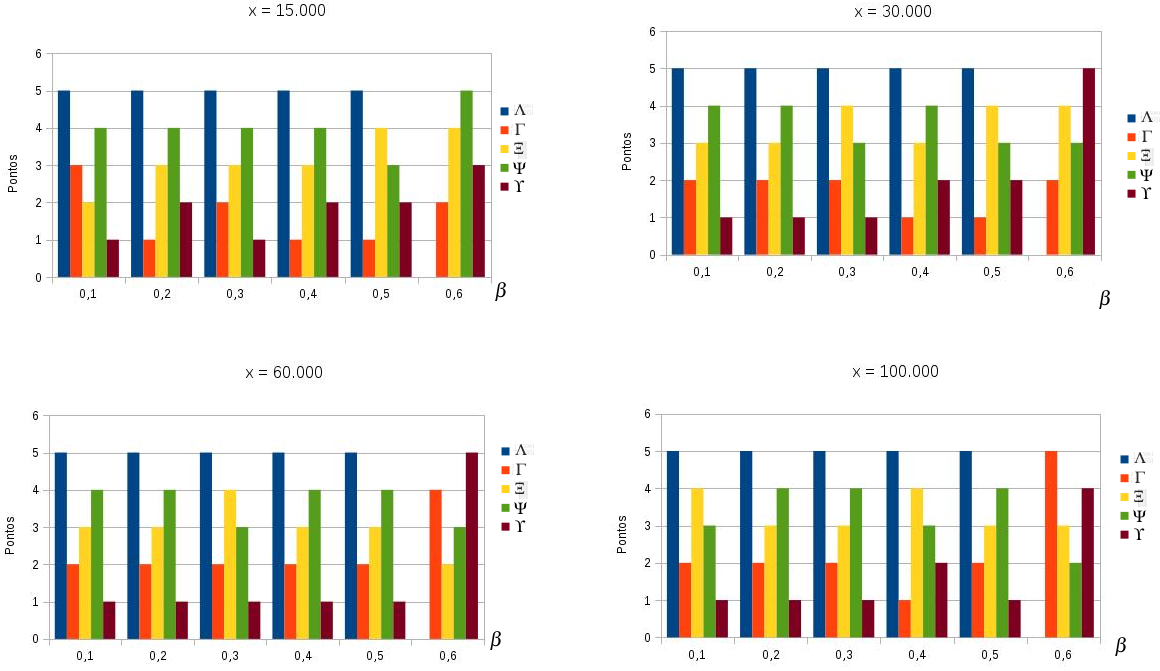
\includegraphics[width=300pt]{imagens_resultados/total_vertices.png}
  \caption{\footnotesize{Pontuação referente ao total de vértices para malhas com $\chi = 15.000$, $\chi = 30.000$, $\chi = 60.000$ e $\chi = 100.000$, com $\beta = 0,1$,
 $\beta = 0,2$, $\beta = 0,3$, $\beta = 0,4$, $\beta = 0,5$ e $\beta = 0,6$.
 \label{grafico_total_vertices}
}}
\end{figure}

\begin{figure}[!ht]
  \centering
  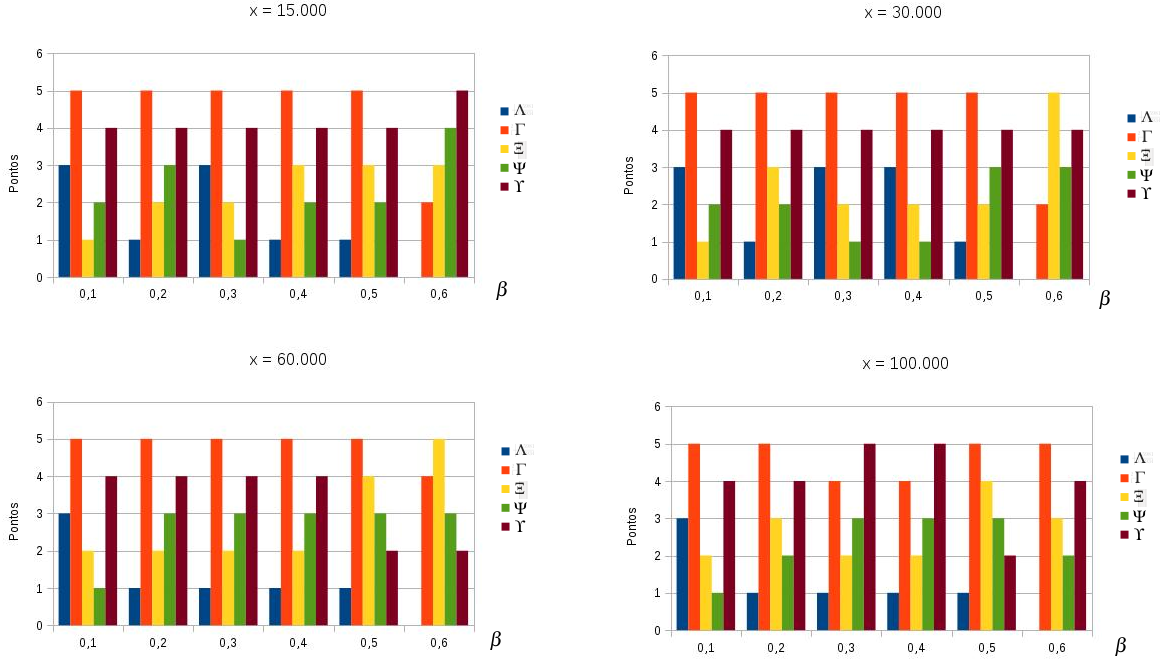
\includegraphics[width=300pt]{imagens_resultados/total_clocks.png}
  \caption{\footnotesize{Pontuação referente ao total de {\it clocks} para malhas com $\chi = 15.000$, $\chi = 30.000$, $\chi = 60.000$ e $\chi = 100.000$, com $\beta = 0,1$, $\beta = 0,2$, $\beta = 0,3$, $\beta = 0,4$, $\beta = 0,5$ e $\beta = 0,6$.
   \label{grafico_total_clocks}
}}
\end{figure}

\begin{figure}[!ht]
  \centering
  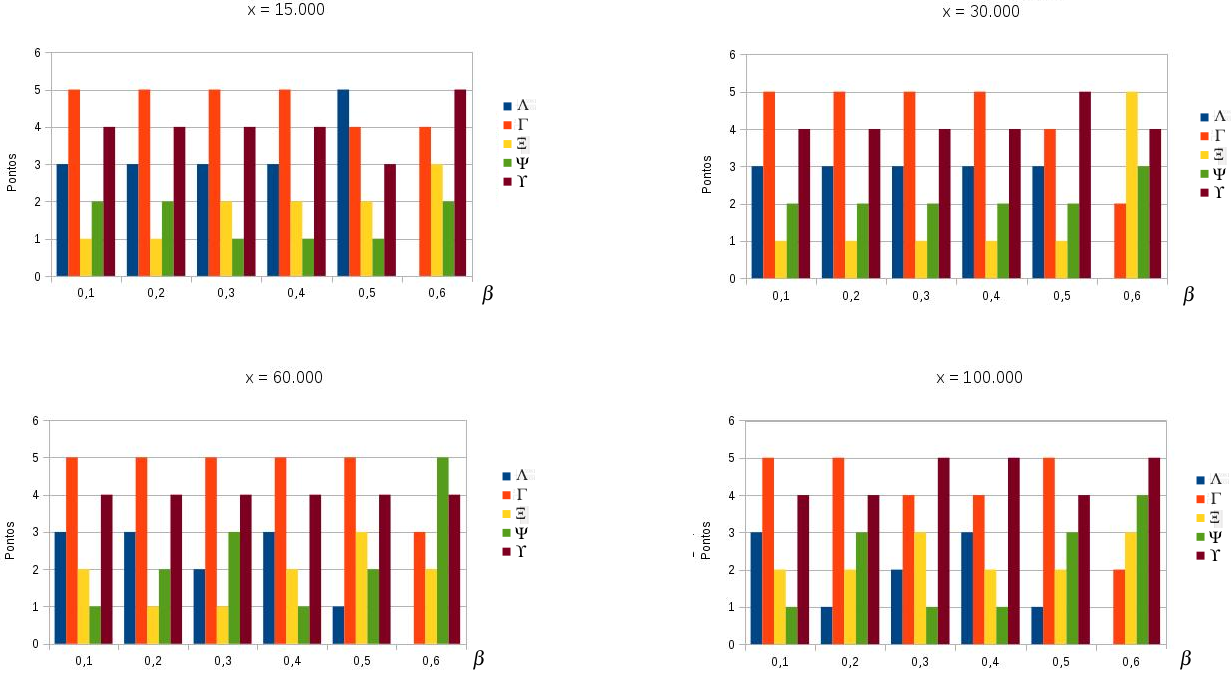
\includegraphics[width=300pt]{imagens_resultados/clocks_mov.png}
  \caption{\footnotesize{Pontuação referente ao total de {\it clocks} para movimentar os vértices, para malhas com $\chi = 15.000$, $\chi = 30.000$, $\chi = 60.000$ e $\chi = 100.000$, com $\beta = 0,1$, $\beta = 0,2$, $\beta = 0,3$, $\beta = 0,4$, $\beta = 0,5$ e $\beta = 0,6$.
   \label{grafico_total_mov}
}}
\end{figure}

\begin{figure}[!ht]
  \centering
  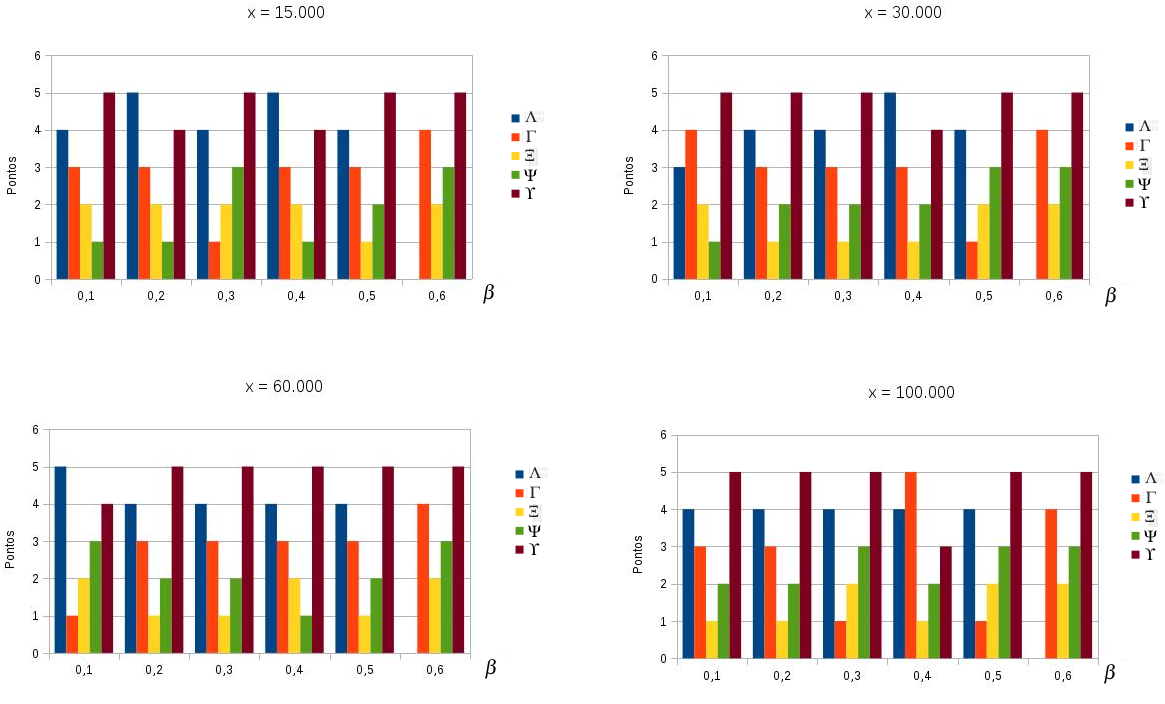
\includegraphics[width=300pt]{imagens_resultados/gamma_max.png}
  \caption{\footnotesize{Pontuação referente ao valor de $\gamma_{max}$, para malhas com $\chi = 15.000$, $\chi = 30.000$, $\chi = 60.000$ e $\chi = 100.000$, com $\beta = 0,1$, $\beta = 0,2$, $\beta = 0,3$, $\beta = 0,4$, $\beta = 0,5$ e $\beta = 0,6$.
   \label{grafico_gamma_max}
}}
\end{figure}

\begin{figure}[!ht]
  \centering
  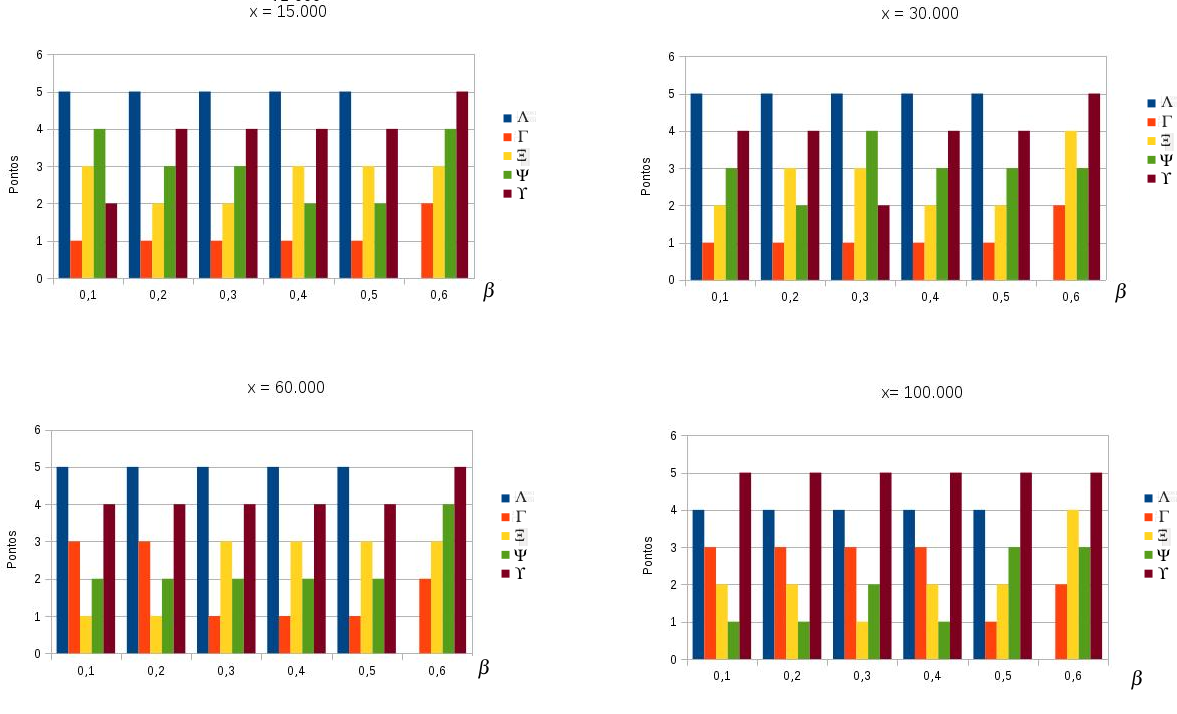
\includegraphics[width=300pt]{imagens_resultados/gamma_mean.png}
  \caption{\footnotesize{Pontuação referente ao valor de $\gamma_{mean}$, para malhas com $\chi = 15.000$, $\chi = 30.000$, $\chi = 60.000$ e $\chi = 100.000$, com $\beta = 0,1$, $\beta = 0,2$, $\beta = 0,3$, $\beta = 0,4$, $\beta = 0,5$ e $\beta = 0,6$.
   \label{grafico_gamma_mean}
}}
\end{figure}

\begin{figure}[!ht]
  \centering
  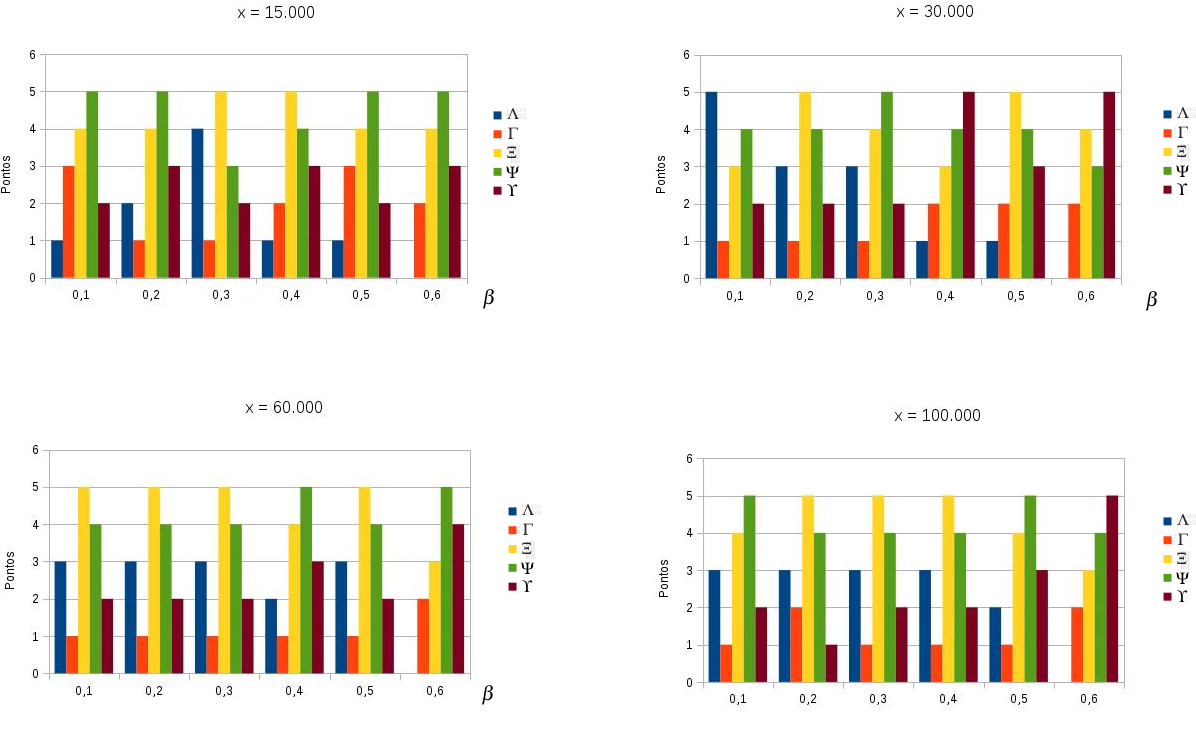
\includegraphics[width=300pt]{imagens_resultados/rho_max.png}
  \caption{\footnotesize{Pontuação referente ao valor de $\rho_{max}$, para malhas com $\chi = 15.000$, $\chi = 30.000$, $\chi = 60.000$ e $\chi = 100.000$, com $\beta = 0,1$, $\beta = 0,2$, $\beta = 0,3$, $\beta = 0,4$, $\beta = 0,5$ e $\beta = 0,6$.
   \label{grafico_rho_max}
}}
\end{figure}

\begin{figure}[!ht]
  \centering
  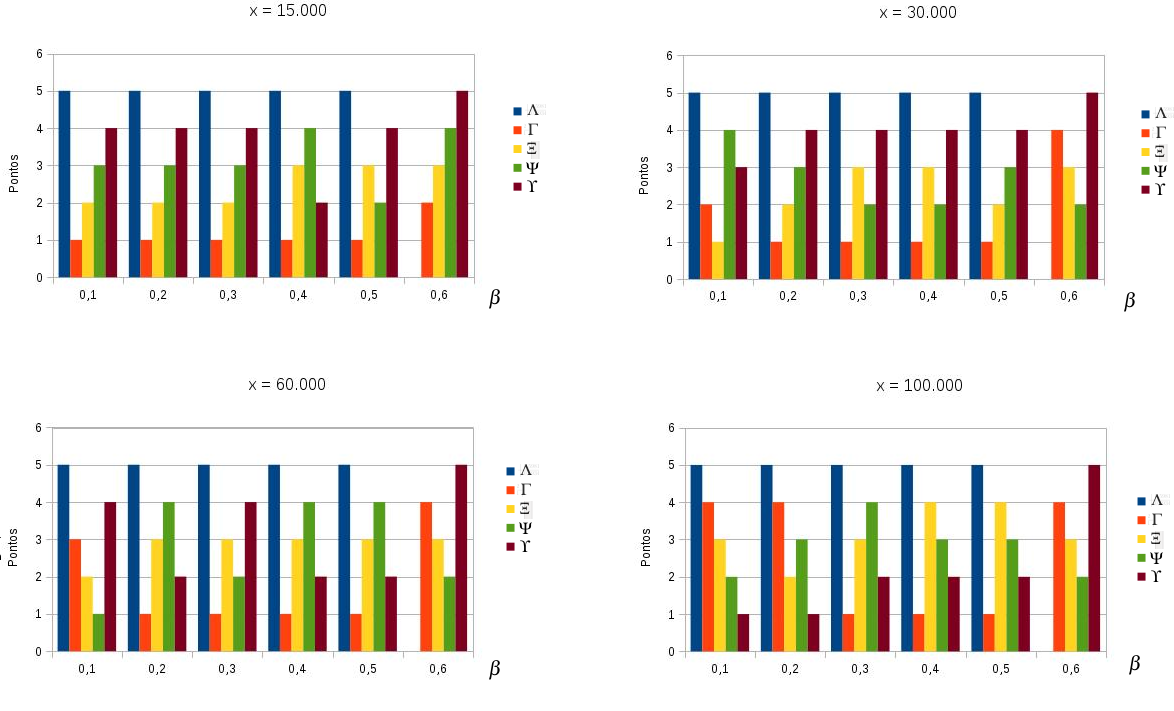
\includegraphics[width=300pt]{imagens_resultados/per_rho.png}
  \caption{\footnotesize{Pontuação referente à porcentagem de triângulos com $\rho > \rho_{\alpha}$, para malhas com $\chi = 15.000$, $\chi = 30.000$, $\chi = 60.000$ e $\chi = 100.000$, com $\beta = 0,1$, $\beta = 0,2$, $\beta = 0,3$, $\beta = 0,4$, $\beta = 0,5$ e $\beta = 0,6$.
   \label{grafico_per_rho}
}}
\end{figure}

\begin{figure}[!ht]
  \centering
  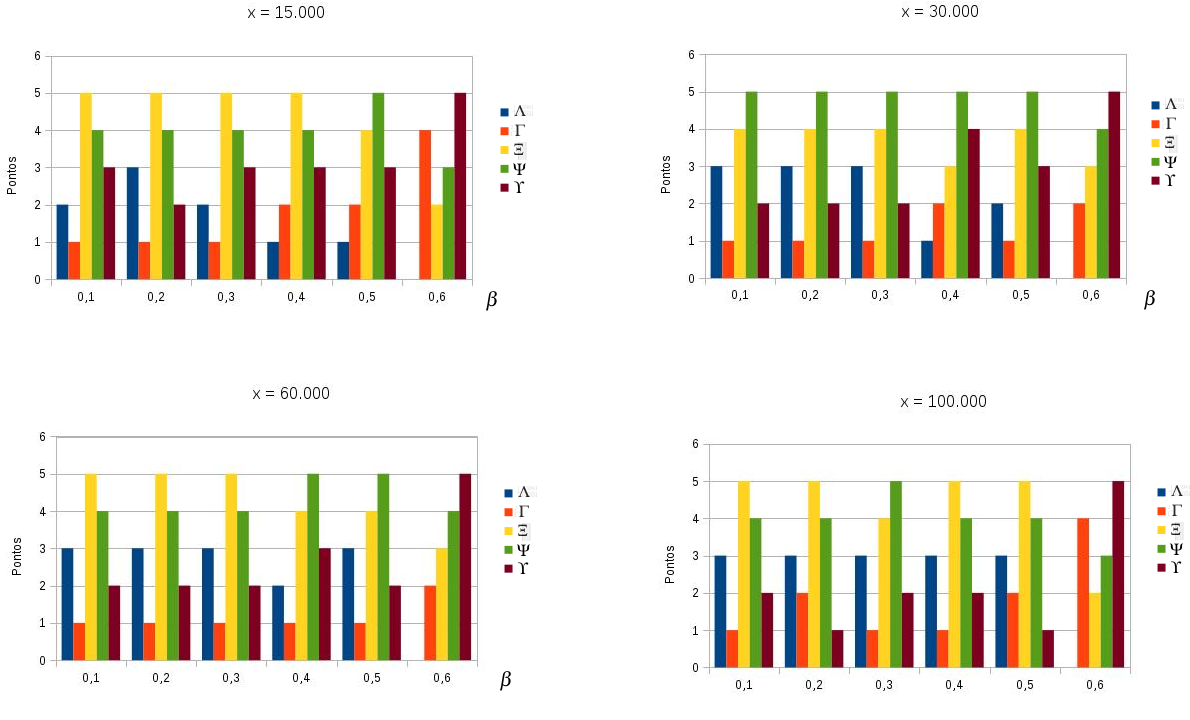
\includegraphics[width=300pt]{imagens_resultados/upsilon_min.png}
  \caption{\footnotesize{Pontuação referente ao valor de $\upsilon_{min}$, para malhas com $\chi = 15.000$, $\chi = 30.000$, $\chi = 60.000$ e $\chi = 100.000$, com $\beta = 0,1$, $\beta = 0,2$, $\beta = 0,3$, $\beta = 0,4$, $\beta = 0,5$ e $\beta = 0,6$.
   \label{grafico_upsilon_min}
}}
\end{figure}

\begin{figure}[!ht]
  \centering
  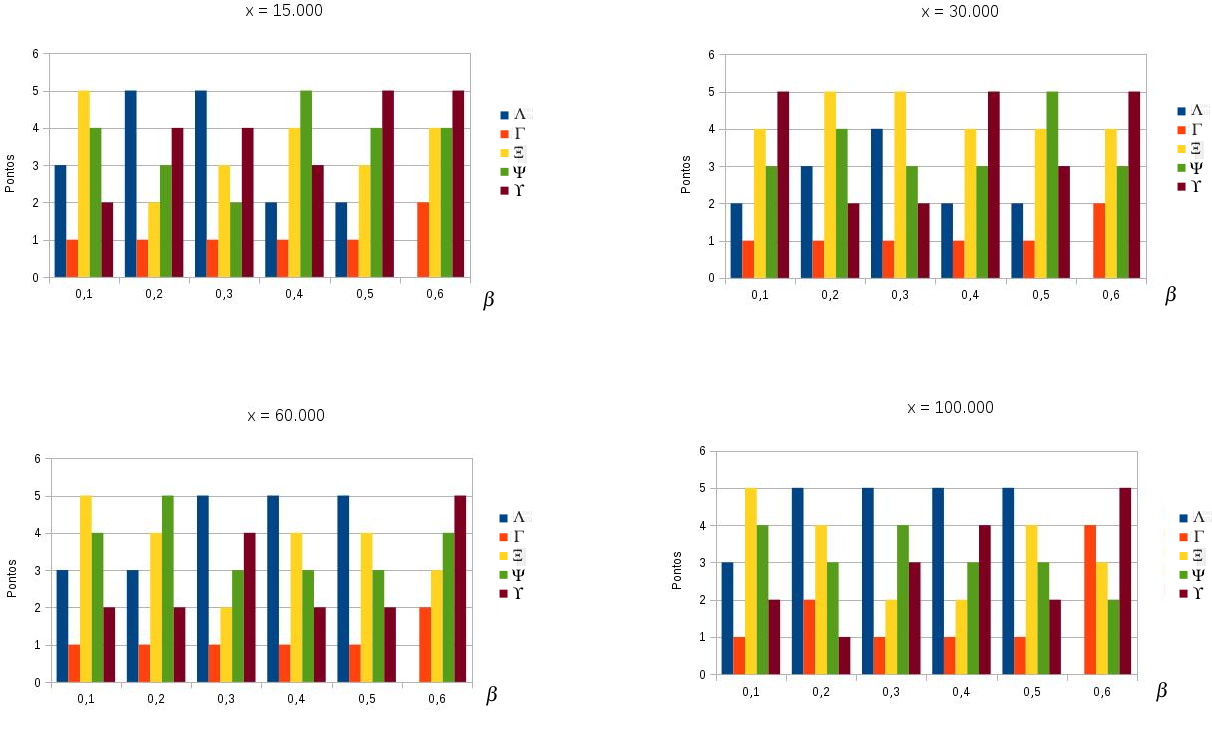
\includegraphics[width=300pt]{imagens_resultados/per_upsilon.png}
  \caption{\footnotesize{Pontuação referente à porcentagem de triângulos com $\upsilon < \eta$, para malhas com $\chi = 15.000$, $\chi = 30.000$, $\chi = 60.000$ e $\chi = 100.000$, com $\beta = 0,1$, $\beta = 0,2$, $\beta = 0,3$, $\beta = 0,4$, $\beta = 0,5$ e $\beta = 0,6$.
   \label{grafico_per_upsilon}
}}
\end{figure}

\begin{figure}[!ht]
  \centering
  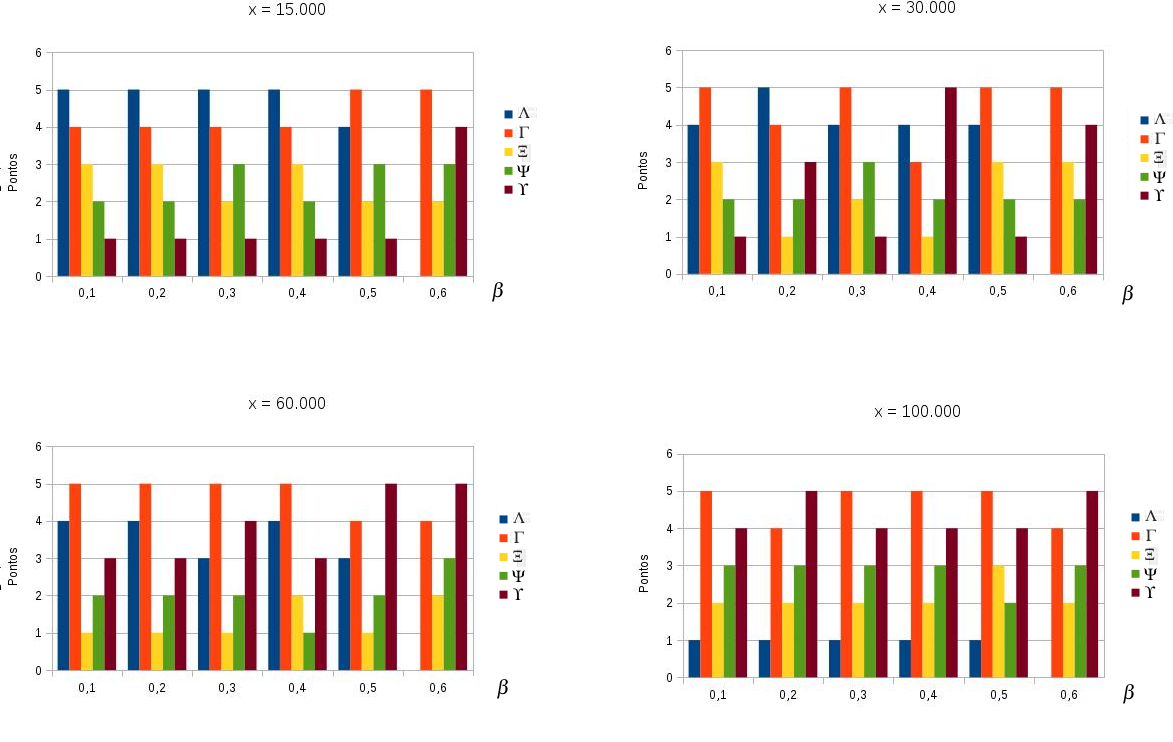
\includegraphics[width=300pt]{imagens_resultados/cresc_gamma.png}
  \caption{\footnotesize{Pontuação referente à porcentagem de crescimento de $\gamma_{mean}$, para malhas com $\chi = 15.000$, $\chi = 30.000$, $\chi = 60.000$ e $\chi = 100.000$, com $\beta = 0,1$, $\beta = 0,2$, $\beta = 0,3$, $\beta = 0,4$, $\beta = 0,5$ e $\beta = 0,6$.
   \label{grafico_cresc_gamma}
}}
\end{figure}